\documentclass[12pt, a4paper]{article}

% 中文支持
\usepackage[UTF8]{ctex}
\usepackage{geometry}
\geometry{left=2cm, right=2cm, top=2.5cm, bottom=2.5cm}

% 图片
\usepackage{graphicx}
\usepackage{float}
\usepackage{subcaption}

% 颜色与样式
\usepackage{xcolor}
\usepackage[framemethod=tikz]{mdframed}
\usepackage{enumitem}
\usepackage{titlesec}
\usepackage{fancyhdr}
\usepackage{hyperref}
\usepackage{tabularx}
\usepackage{booktabs}
\usepackage{fontspec}
\usepackage{setspace}

% 定义颜色
\definecolor{meituan}{RGB}{255, 198, 0}
\definecolor{darktext}{RGB}{51, 51, 51}
\definecolor{graytext}{RGB}{102, 102, 102}
\definecolor{painred}{RGB}{220, 53, 69}
\definecolor{hopegreen}{RGB}{40, 167, 69}
\definecolor{softbg}{RGB}{248, 249, 250}

% mdframed 样式定义
\mdfdefinestyle{storystyle}{
    backgroundcolor=softbg,
    linewidth=0pt,
    roundcorner=6pt,
    innertopmargin=12pt,
    innerbottommargin=12pt,
    innerleftmargin=15pt,
    innerrightmargin=15pt
}
\mdfdefinestyle{painstyle}{
    backgroundcolor=painred!5,
    linecolor=painred!30,
    linewidth=0.5pt,
    roundcorner=6pt,
    innertopmargin=12pt,
    innerbottommargin=12pt,
    innerleftmargin=15pt,
    innerrightmargin=15pt,
    frametitlebackgroundcolor=painred!10,
    frametitlerulewidth=0pt
}
\mdfdefinestyle{hopestyle}{
    backgroundcolor=hopegreen!5,
    linecolor=hopegreen!40,
    linewidth=0.5pt,
    roundcorner=6pt,
    innertopmargin=12pt,
    innerbottommargin=12pt,
    innerleftmargin=15pt,
    innerrightmargin=15pt
}
\mdfdefinestyle{infostyle}{
    backgroundcolor=meituan!8,
    linecolor=meituan!60,
    linewidth=0.5pt,
    roundcorner=6pt,
    innertopmargin=12pt,
    innerbottommargin=12pt,
    innerleftmargin=15pt,
    innerrightmargin=15pt
}
\mdfdefinestyle{flowstyle}{
    backgroundcolor=softbg,
    linecolor=graytext!30,
    linewidth=0.3pt,
    roundcorner=6pt,
    innertopmargin=15pt,
    innerbottommargin=15pt,
    innerleftmargin=15pt,
    innerrightmargin=15pt
}
\mdfdefinestyle{endstyle}{
    backgroundcolor=meituan!10,
    linecolor=meituan!70,
    linewidth=0.5pt,
    roundcorner=8pt,
    innertopmargin=15pt,
    innerbottommargin=15pt,
    innerleftmargin=20pt,
    innerrightmargin=20pt
}

% 标题样式
\titleformat{\section}{\Large\bfseries\color{darktext}}{}{0em}{}
\titleformat{\subsection}{\large\bfseries\color{graytext}}{}{0em}{}

% 页眉页脚
\pagestyle{fancy}
\fancyhf{}
\fancyhead[L]{\small\color{graytext}实时探路 · 产品说明文档}
\fancyhead[R]{\small\color{graytext}\thepage}
\renewcommand{\headrulewidth}{0.4pt}
\setlength{\headheight}{14pt}

% 超链接样式
\hypersetup{
    colorlinks=true,
    linkcolor=darktext,
    urlcolor=meituan
}

% 行间距
\setstretch{1.5}

% 图片路径
\graphicspath{{图片/}{实时探路/}}

\begin{document}

% ========== 封面 ==========
\begin{titlepage}
\centering
\vspace*{3cm}

{\Huge\bfseries 实时探路}\\[0.5cm]
{\LARGE\color{graytext} 出发之前，先看一眼}\\[2cm]

{\large 让每一次出行都不白跑}\\[0.3cm]
{\large\color{graytext} 基于位置的实时信息众包服务平台}\\[4cm]

{\normalsize 版本：v1.0}\\[0.2cm]
{\normalsize \today}

\vfill
\end{titlepage}

% ========== 目录 ==========
\tableofcontents
\newpage

% ============================================================
%   第一章：痛点故事一 —— 动物园
% ============================================================
\section{你一定经历过这样的周末}

\begin{mdframed}[style=storystyle]
{\large\itshape "爸爸妈妈！我们去动物园好不好！"}

\vspace{6pt}
周六早上，你刷到了美团上动物园的团购券。孩子听到消息，兴奋得跳了起来。
你们收拾好东西，满怀期待地出发了。
\end{mdframed}

\vspace{0.3cm}

\begin{figure}[H]
    \centering
    \begin{subfigure}[b]{0.32\textwidth}
        
\includegraphics[width=\textwidth]{1刷到了美团团购.png}
        \caption*{刷到了团购券}
    \end{subfigure}
    \hfill
    \begin{subfigure}[b]{0.32\textwidth}
        
\includegraphics[width=\textwidth]{3孩子听到去动物园很开心.png}
        \caption*{孩子兴奋不已}
    \end{subfigure}
    \hfill
    \begin{subfigure}[b]{0.32\textwidth}
        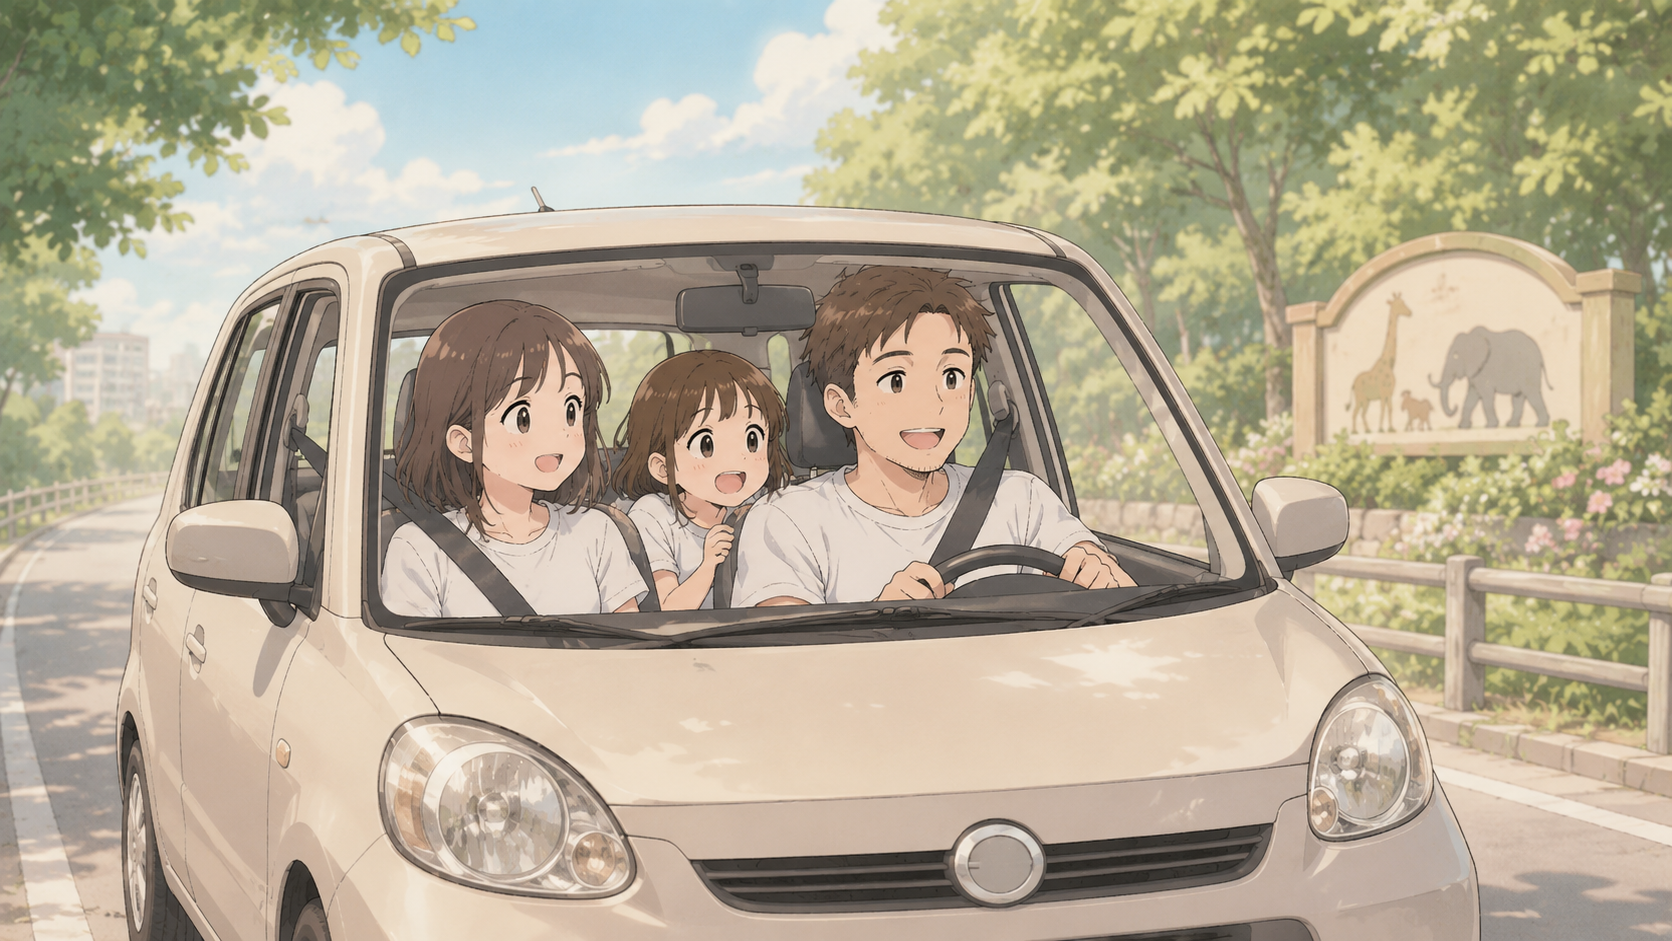
\includegraphics[width=\textwidth]{4一起开车出发.png}
        \caption*{满怀期待出发}
    \end{subfigure}
\end{figure}

\vspace{0.5cm}

% === 到达后的崩溃 ===
{\color{painred}\bfseries \large 然而……}
\begin{mdframed}[style=painstyle]
开了四十分钟的车，终于到了。

可眼前的景象让你心凉了半截——\textbf{人山人海}。停车场满了，门口排着看不到尽头的队伍。太阳暴晒，孩子开始烦躁。你和爱人对视一眼，心里都清楚：今天怕是白来了。

\vspace{6pt}
\textbf{你开始犹豫：}排下去？至少还要一个小时。走？孩子的期待怎么办？

最终你们选择了离开。
\end{mdframed}

\begin{figure}[H]
    \centering
    \begin{subfigure}[b]{0.32\textwidth}
        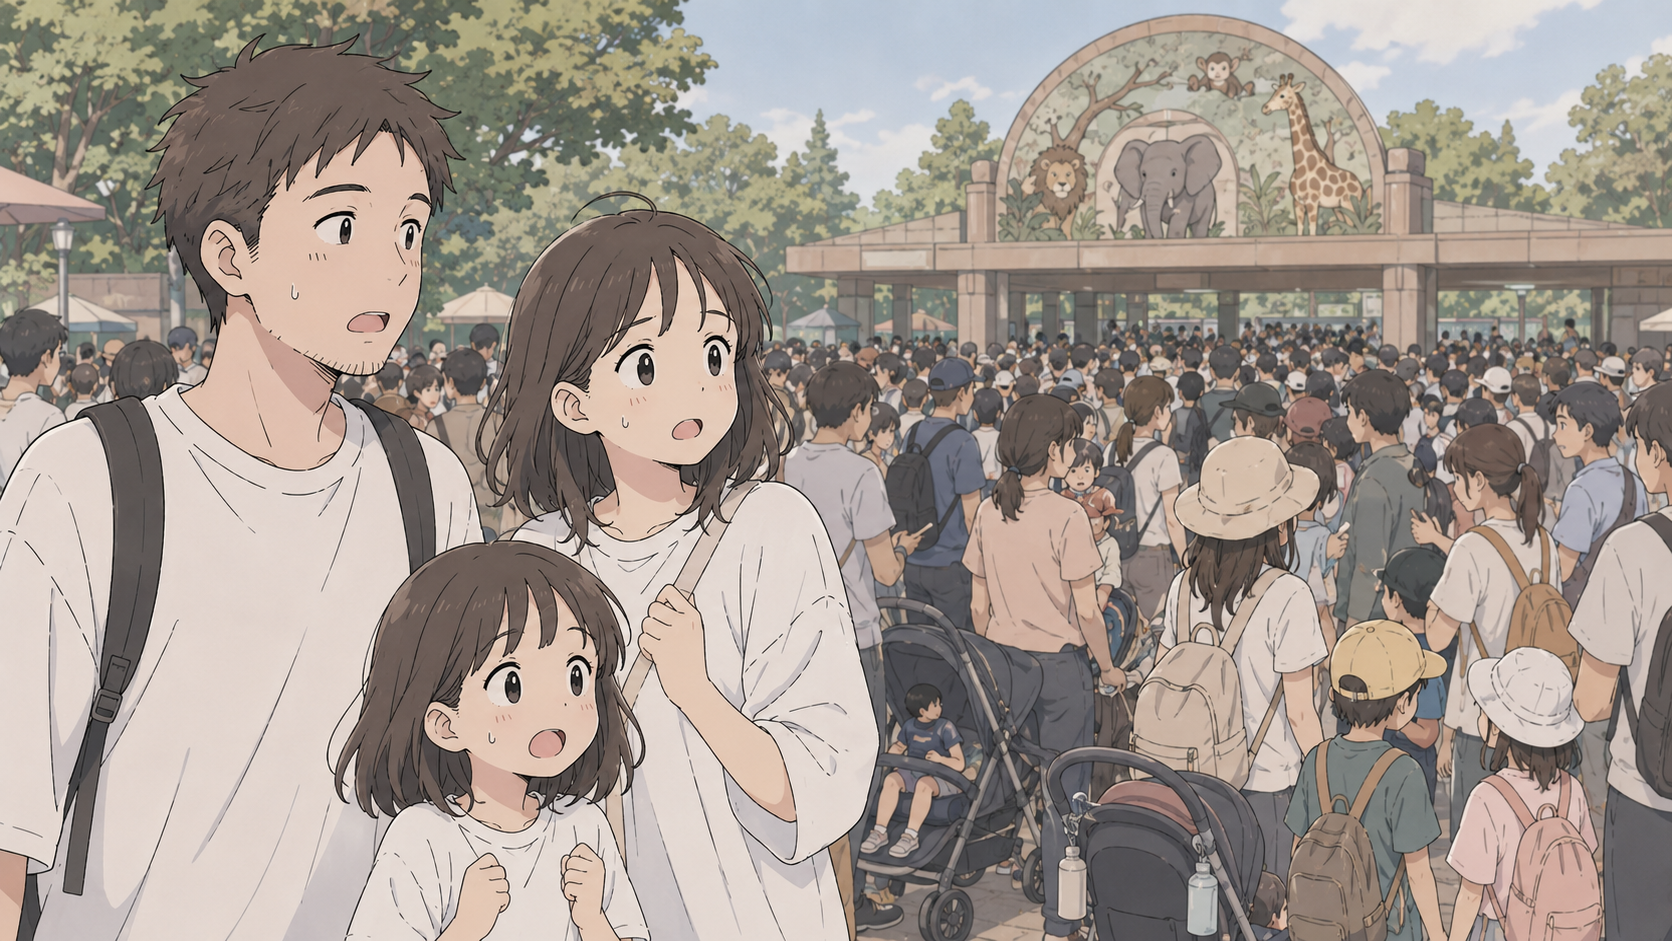
\includegraphics[width=\textwidth]{5到门口发现全是人.png}
        \caption*{到了才发现全是人}
    \end{subfigure}
    \hfill
    \begin{subfigure}[b]{0.32\textwidth}
        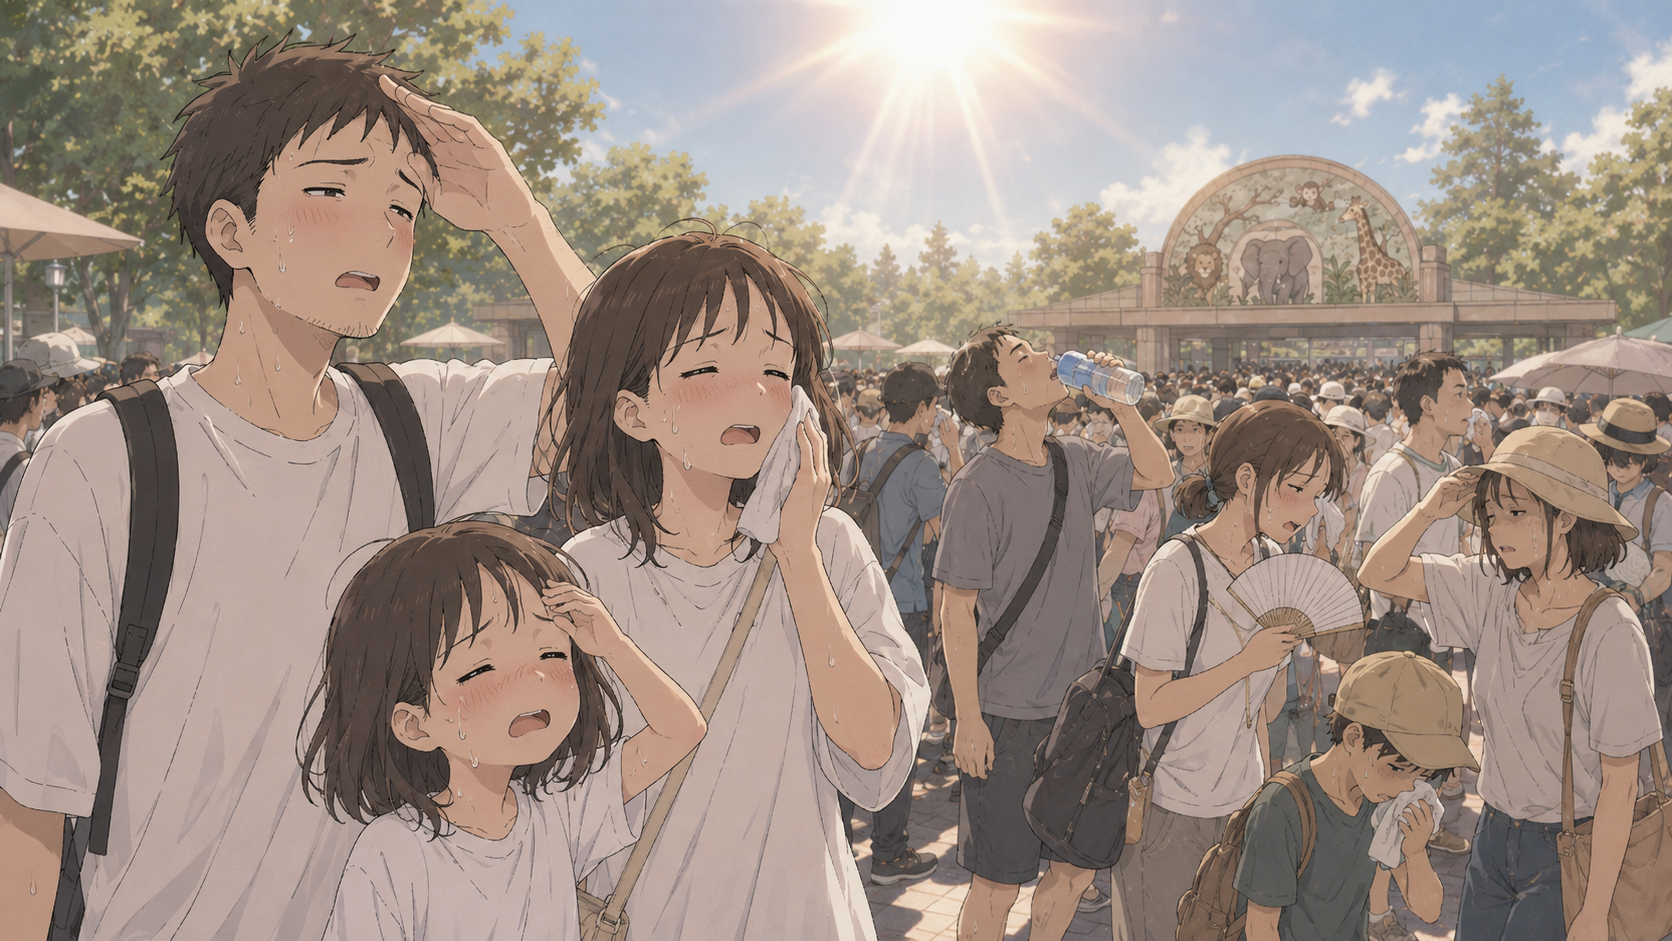
\includegraphics[width=\textwidth]{6人很多很热.png}
        \caption*{烈日暴晒，人潮拥挤}
    \end{subfigure}
    \hfill
    \begin{subfigure}[b]{0.32\textwidth}
        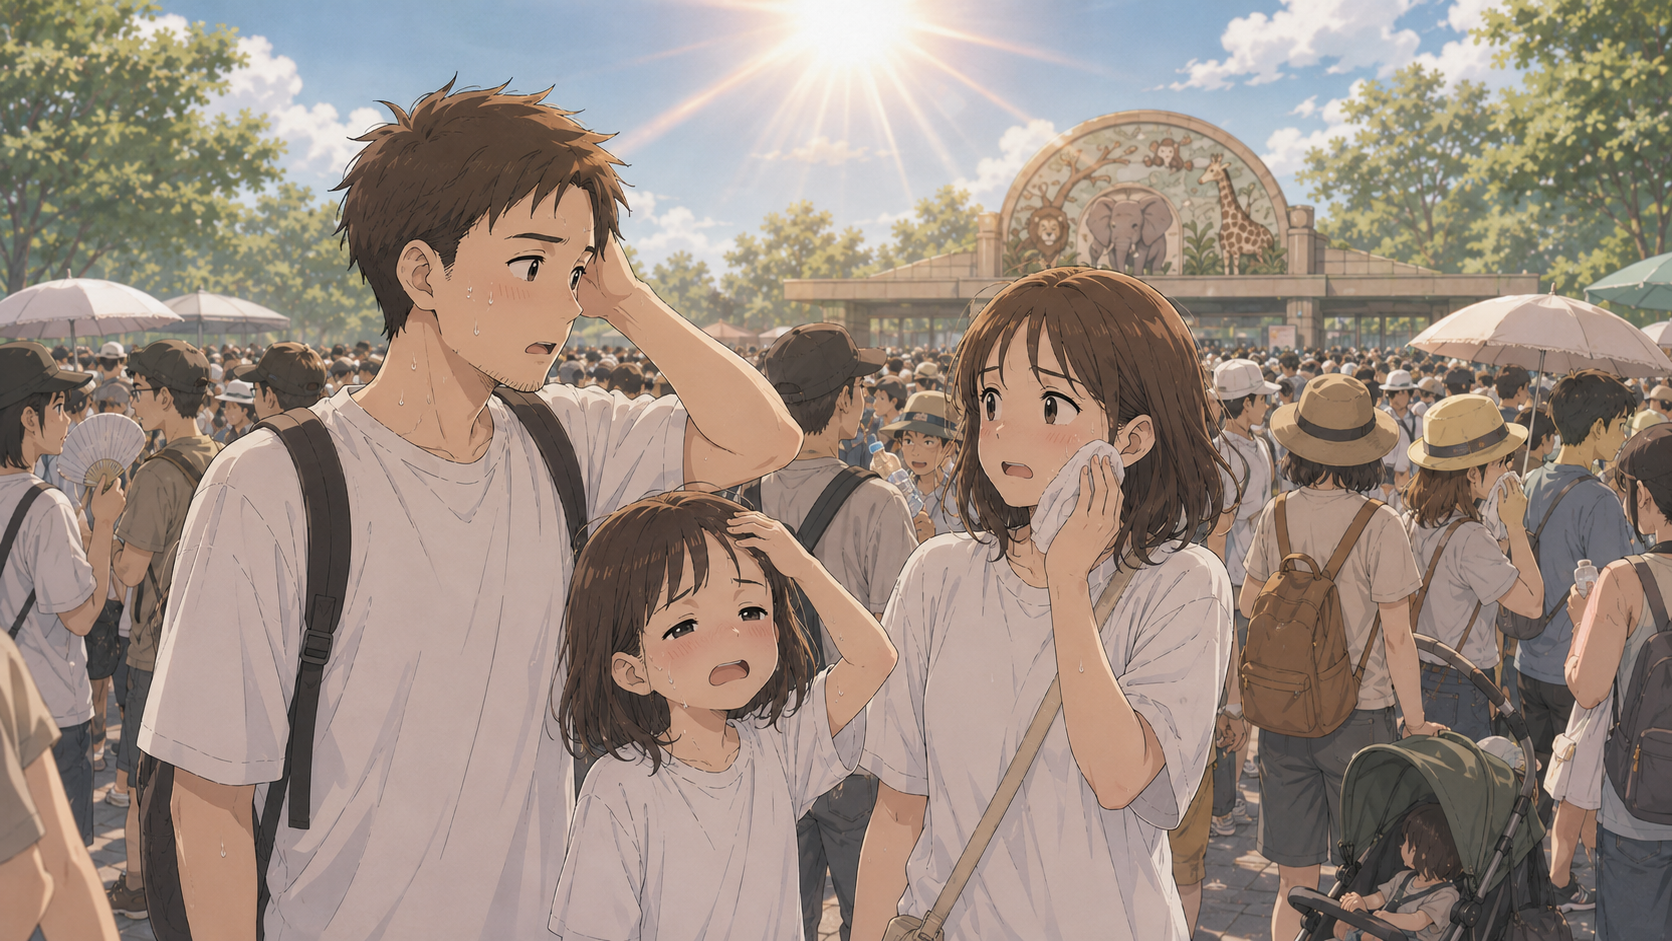
\includegraphics[width=\textwidth]{7父母商量是否需要离开.png}
        \caption*{无奈商量是否离开}
    \end{subfigure}
\end{figure}

\begin{figure}[H]
    \centering
    \begin{subfigure}[b]{0.32\textwidth}
        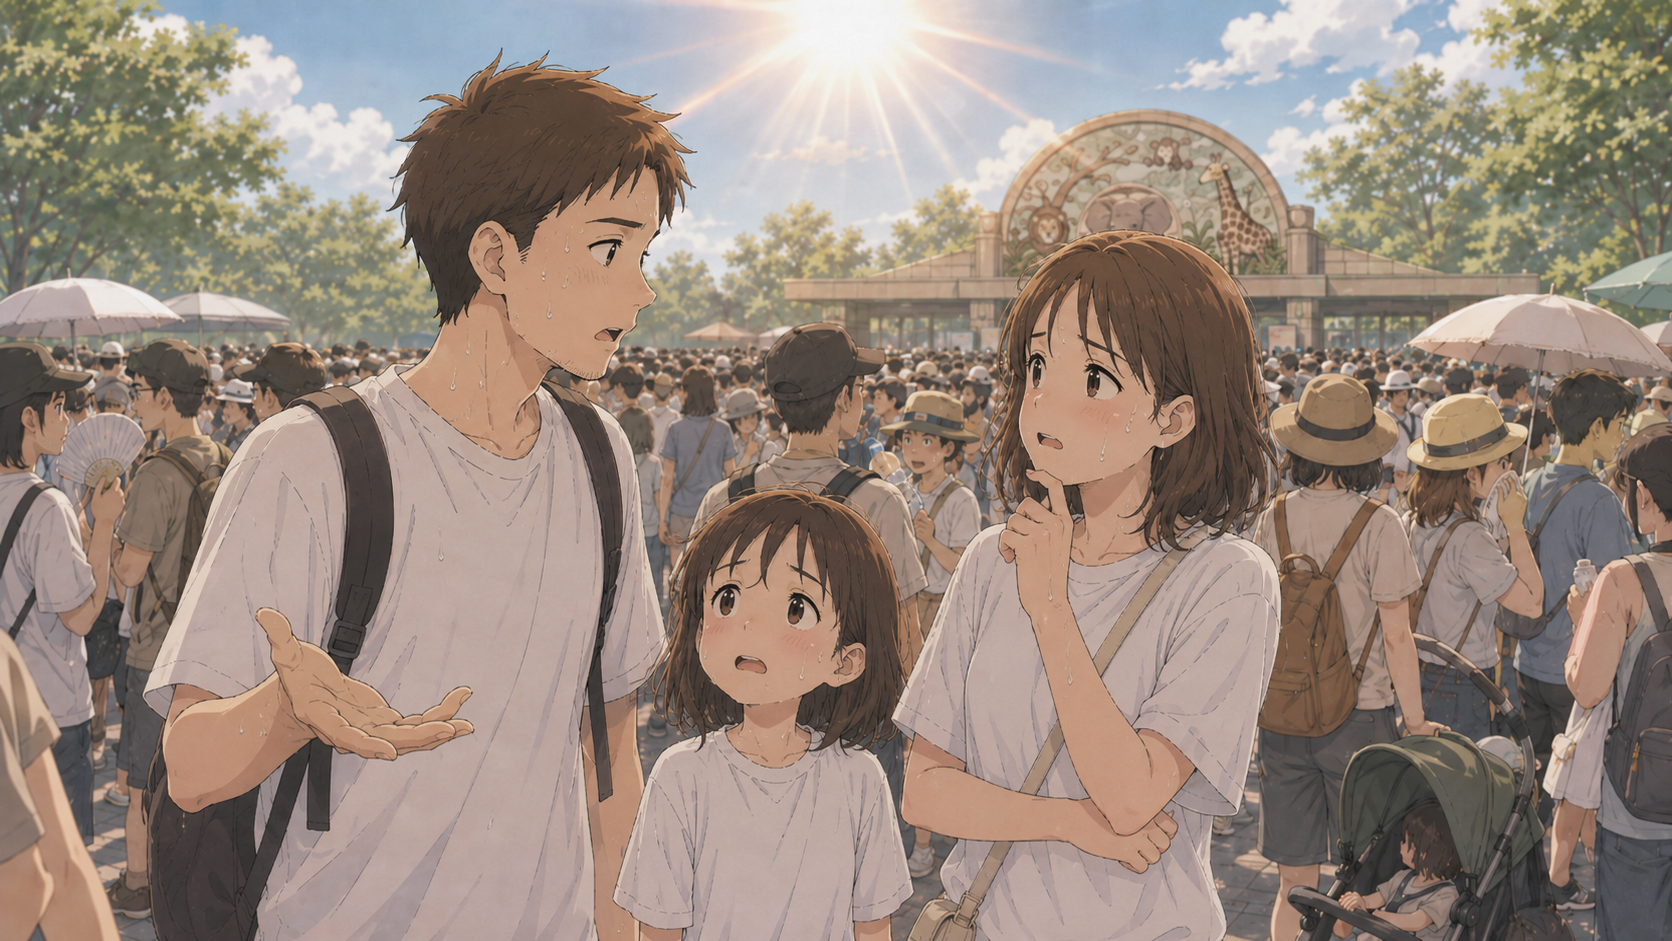
\includegraphics[width=\textwidth]{8担心中暑决定离开.png}
        \caption*{担心中暑，决定离开}
    \end{subfigure}
    \hfill
    \begin{subfigure}[b]{0.32\textwidth}
        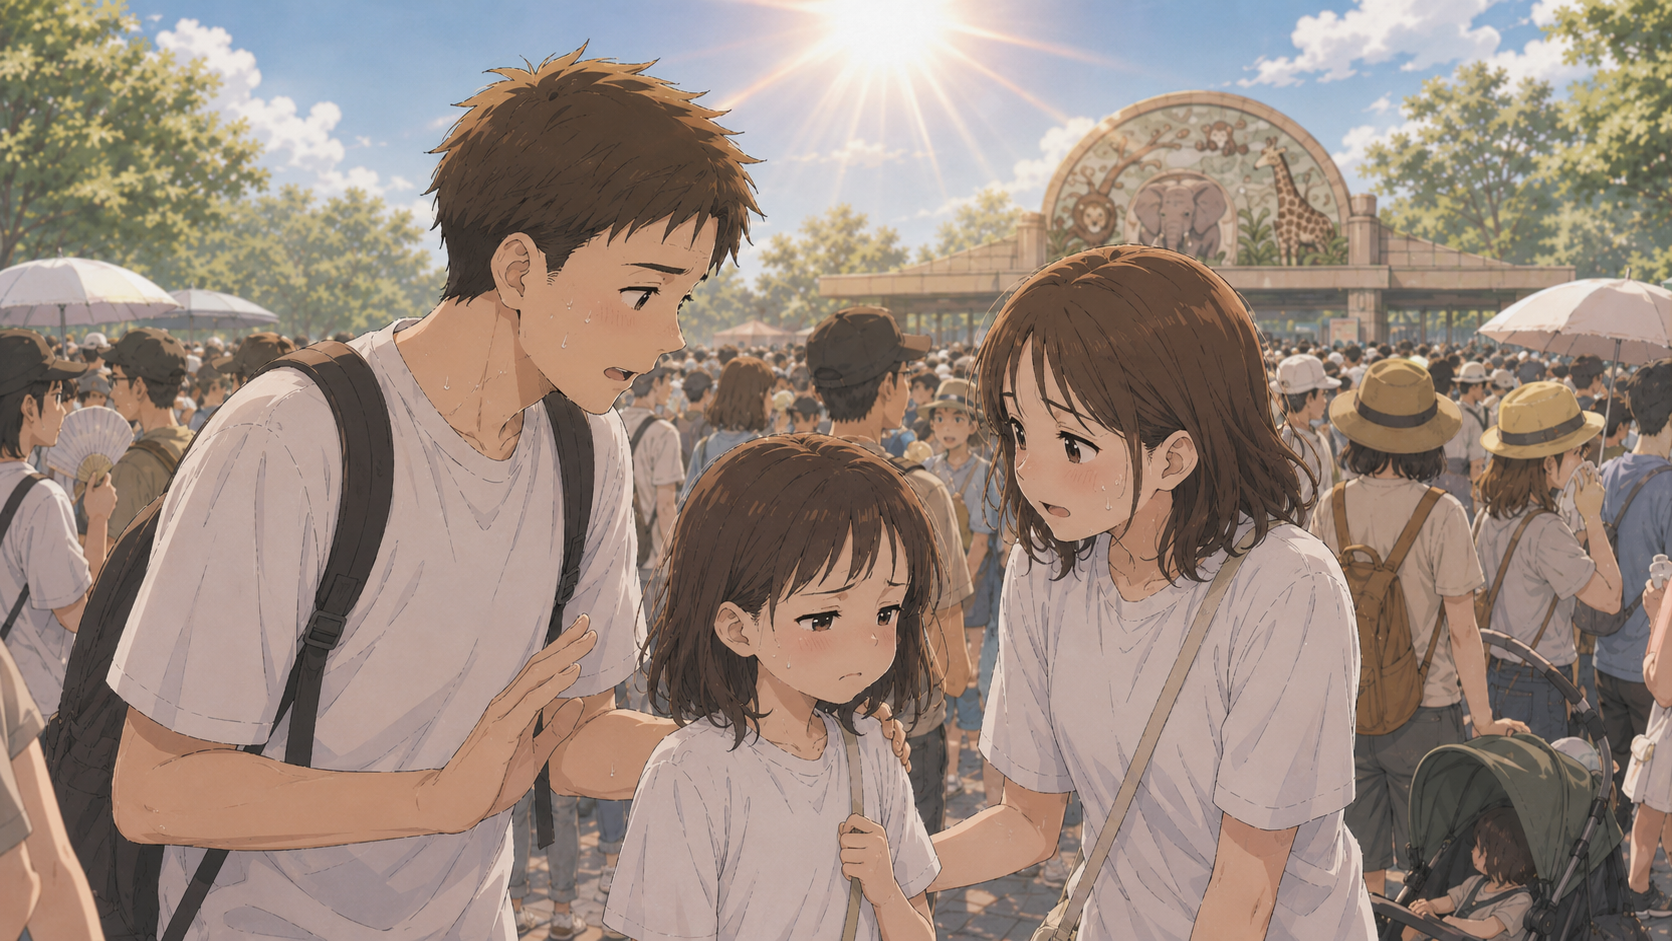
\includegraphics[width=\textwidth]{9孩子伤心.png}
        \caption*{孩子失落的眼神}
    \end{subfigure}
    \hfill
    \begin{subfigure}[b]{0.32\textwidth}
        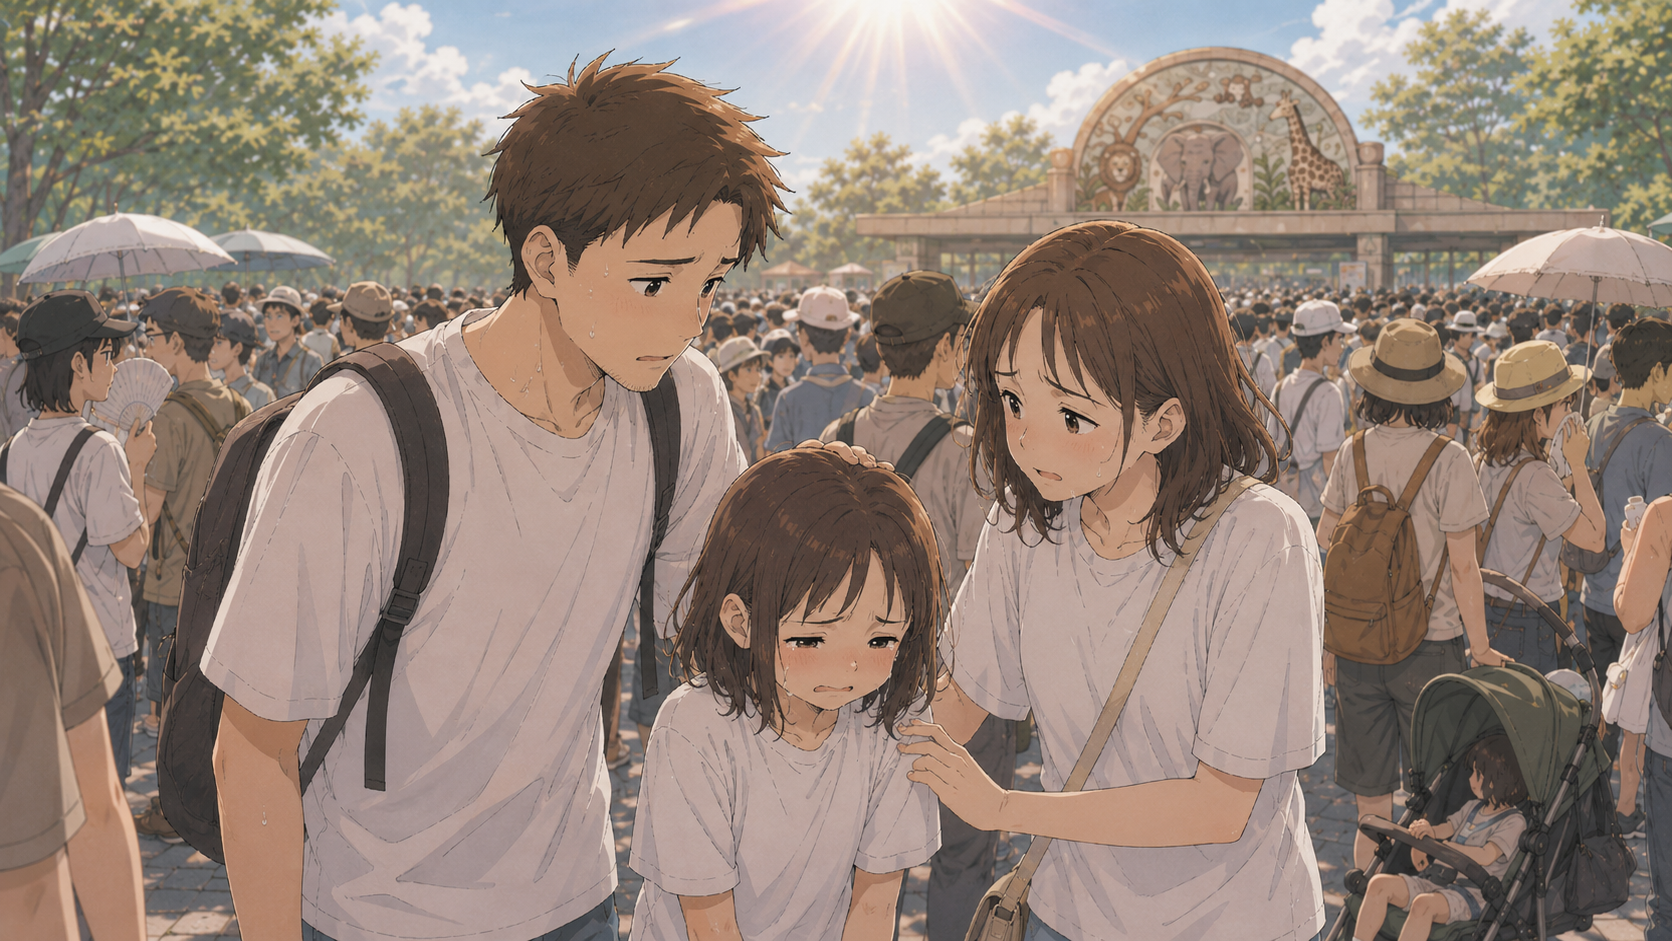
\includegraphics[width=\textwidth]{10孩子哭了.png}
        \caption*{孩子哭了}
    \end{subfigure}
\end{figure}

\vspace{0.3cm}
\begin{center}
{\large\color{painred}\bfseries 浪费的不只是时间和油钱，\\更是孩子满心的期待。}
\end{center}

\begin{figure}[H]
    \centering
    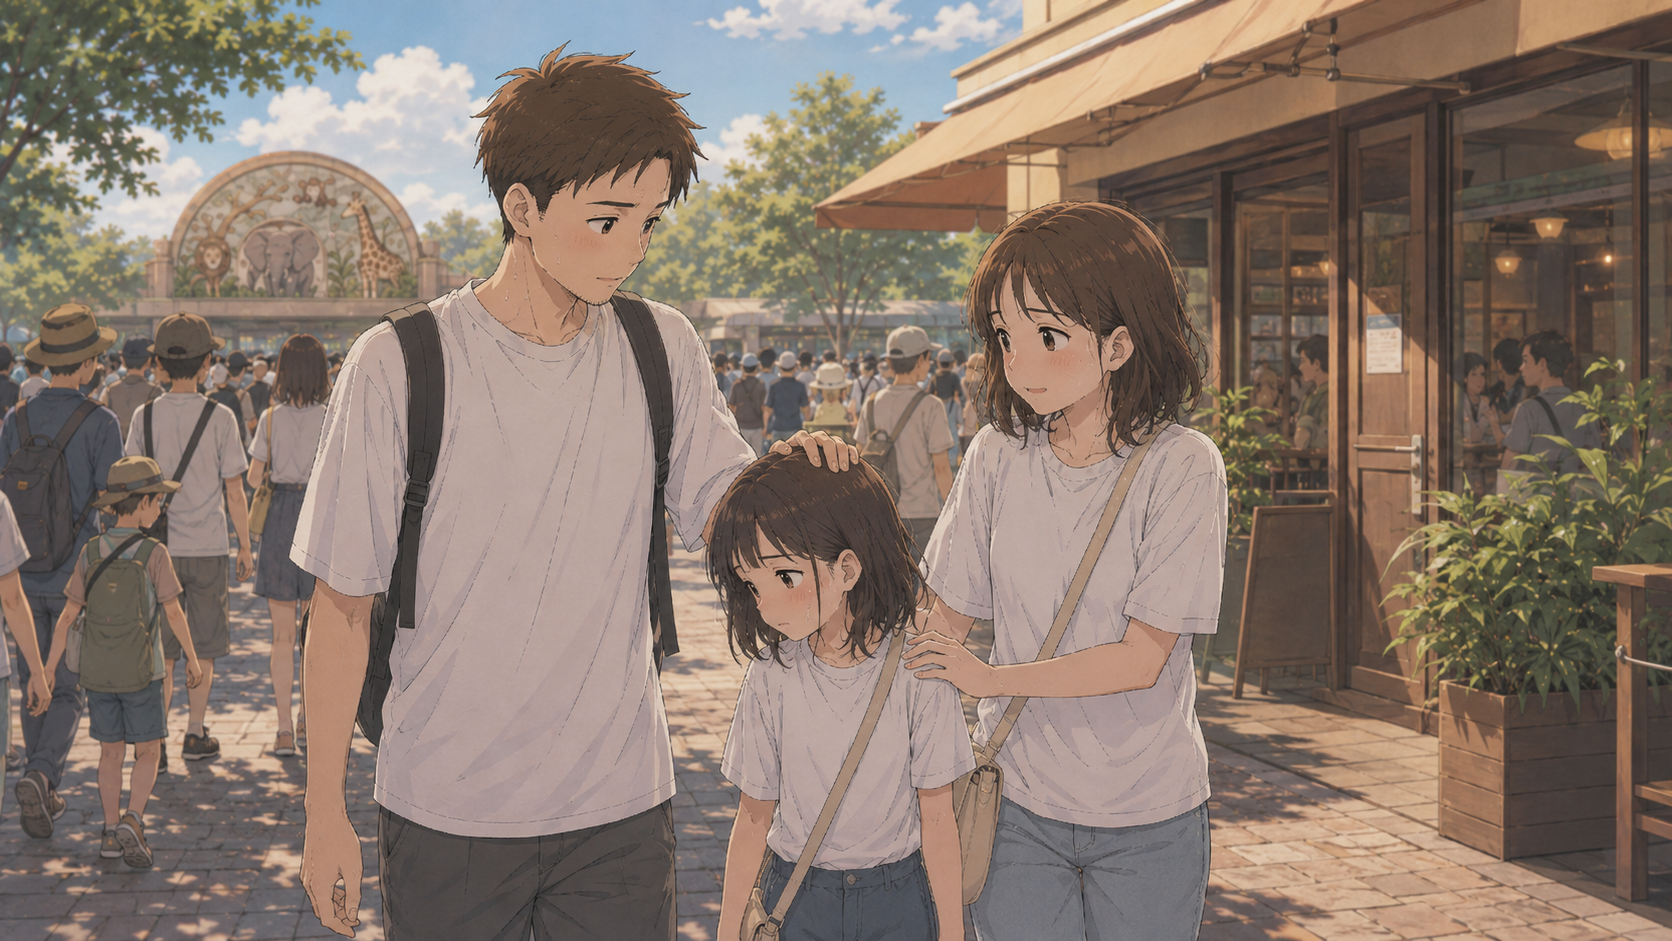
\includegraphics[width=0.4\textwidth]{11孩子依依不舍.png}
    \caption*{\small 孩子回头望着动物园的方向，依依不舍}
\end{figure}

\newpage

% ============================================================
%   第二章：转折
% ============================================================
\section{如果，出发前你就能知道呢？}

{\color{hopegreen}\bfseries \large 让我们倒回出发前的那一刻}
\begin{mdframed}[style=hopestyle]
同样的周六早上，你同样刷到了那张团购券。

但这次，你打开了\textbf{「实时探路」}，发布了一个任务：

\vspace{6pt}
\begin{center}
\itshape "帮我看看动物园现在排队情况怎么样，人多吗？"
\end{center}
\vspace{6pt}

几分钟后，一位刚好在动物园附近的游客接了你的单。他发来了现场照片，并告诉你：

\vspace{6pt}
\begin{center}
\itshape "人超多的，门口排队至少要40分钟，里面也到处是人，建议换个时间来。"
\end{center}
\end{mdframed}

\begin{figure}[H]
    \centering
    \begin{subfigure}[b]{0.32\textwidth}
        
\includegraphics[width=\textwidth]{12当你在出发前使用了实时探路.png}
        \caption*{出发前打开实时探路}
    \end{subfigure}
    \hfill
    \begin{subfigure}[b]{0.32\textwidth}
        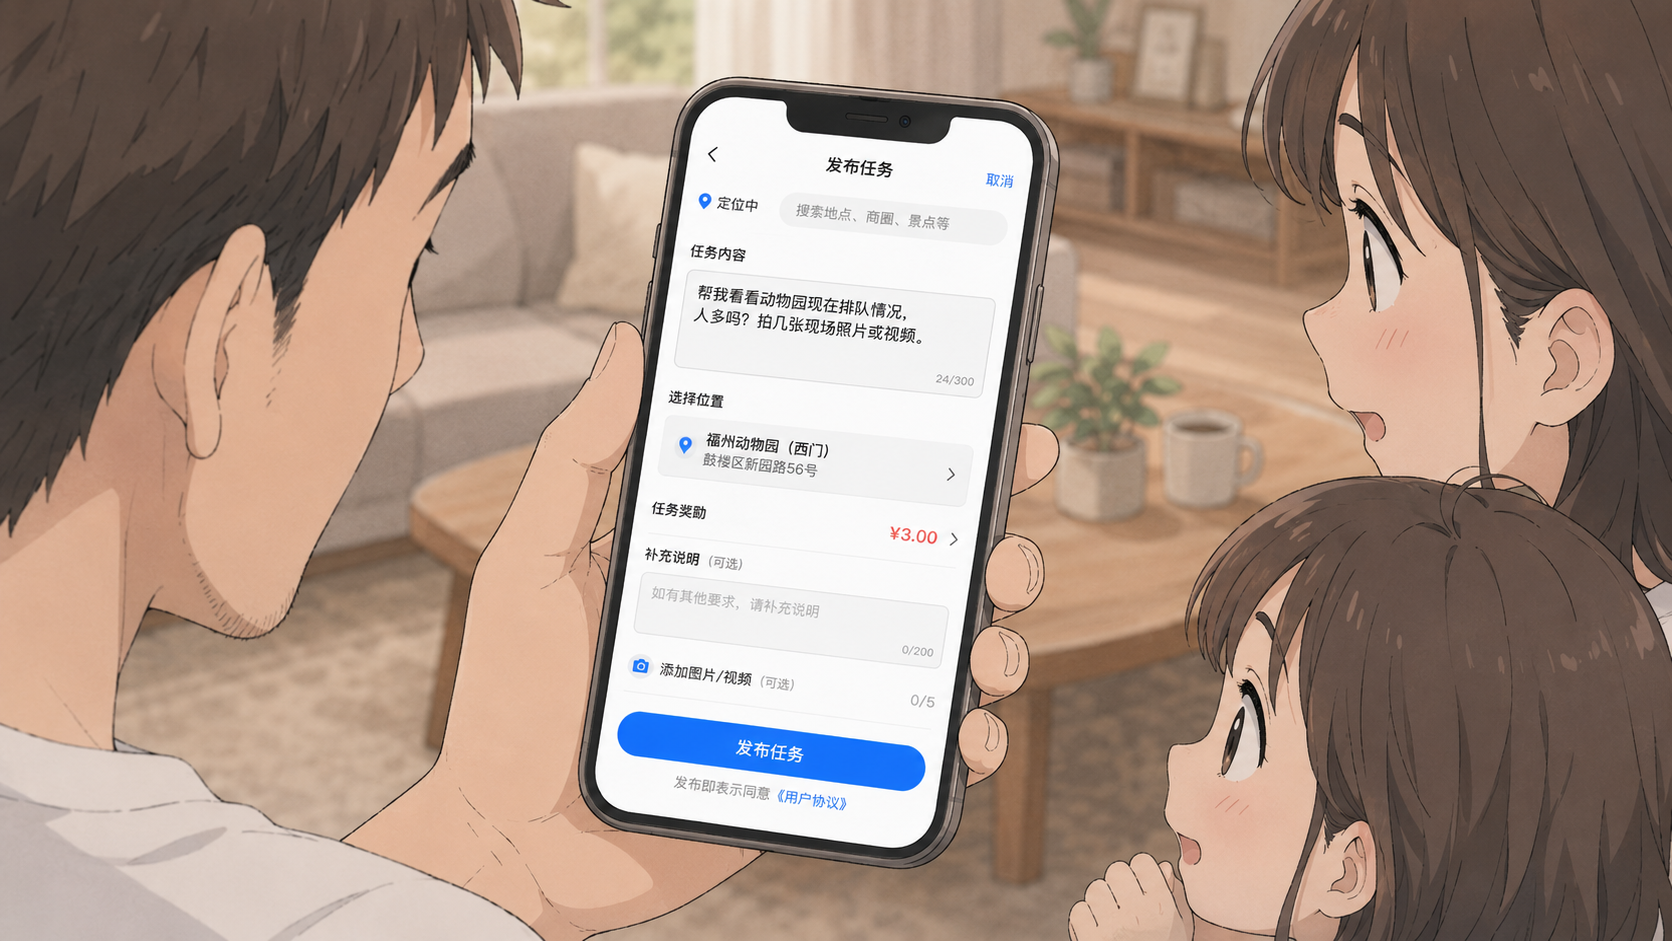
\includegraphics[width=\textwidth]{13你发布了一个任务.png}
        \caption*{发布探路任务}
    \end{subfigure}
    \hfill
    \begin{subfigure}[b]{0.32\textwidth}
        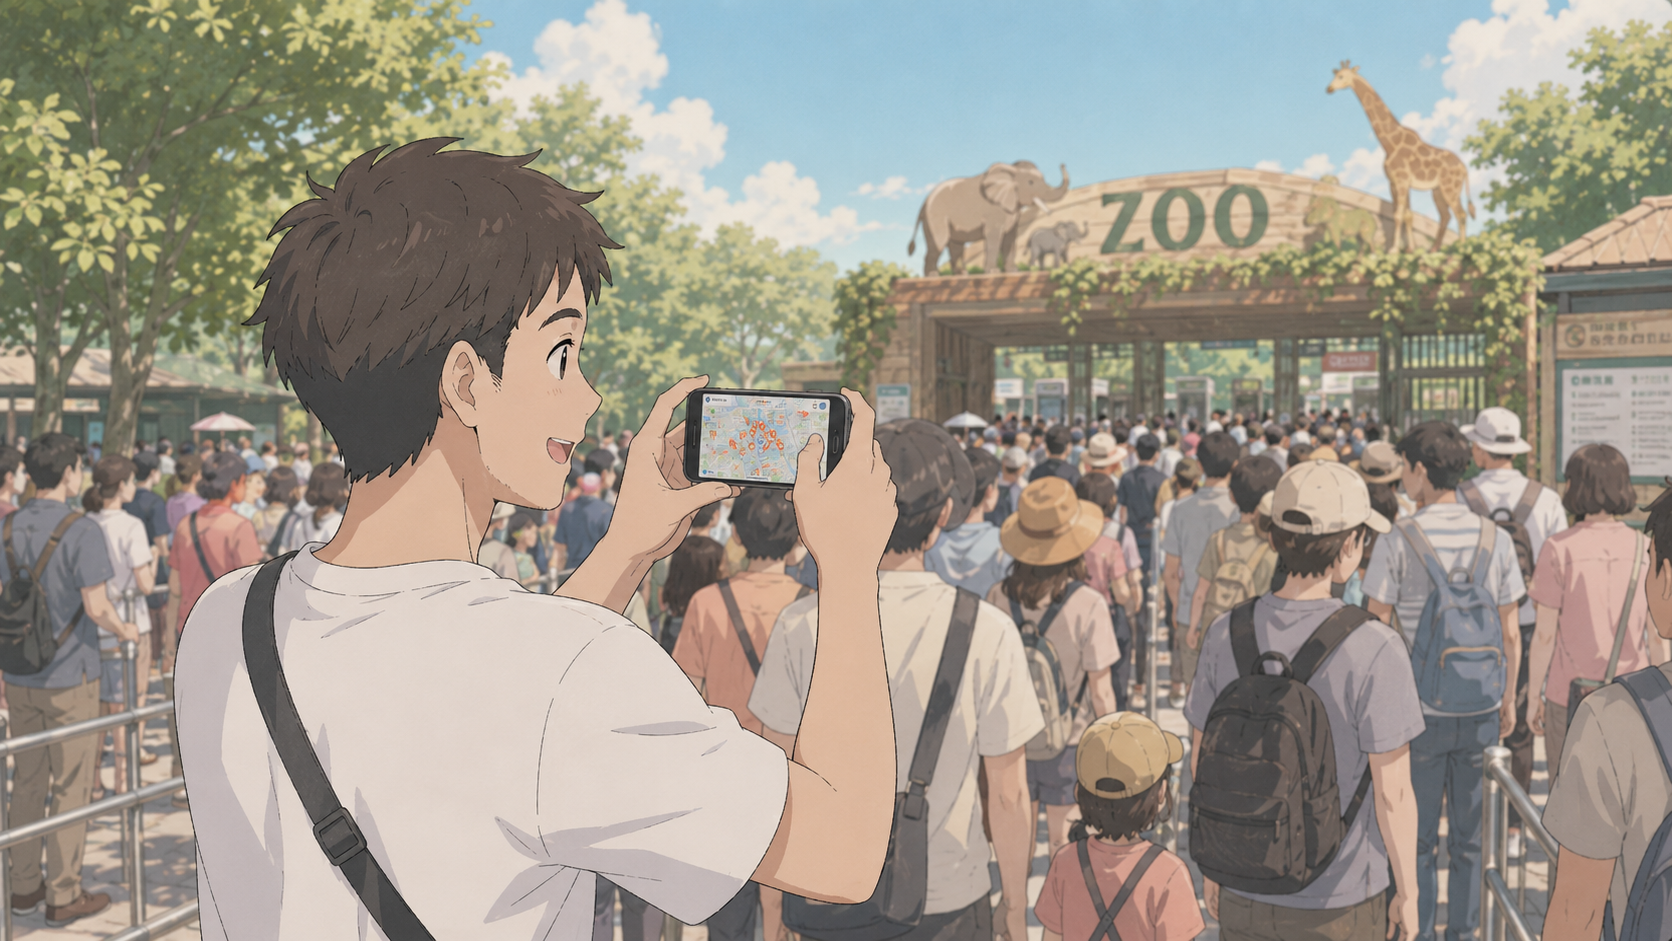
\includegraphics[width=\textwidth]{14刚好在动物园的游客接了你的任务，给你拍照并告诉你人太多了.png}
        \caption*{附近游客帮你拍了现场}
    \end{subfigure}
\end{figure}

\vspace{0.3cm}

\begin{mdframed}[style=hopestyle]
你把这件事告诉了孩子。孩子虽然有点失望，但你们一起商量了新的计划——

\textbf{去郊外野餐！}

你们把原本可能浪费在排队和暴晒上的三个小时，换成了一场轻松愉快的春游。铺上野餐垫，吃着零食，孩子在草地上奔跑，你们一起吃冰淇淋……

\vspace{6pt}
{\large\color{hopegreen}\bfseries 同样的周末，完全不同的结局。}
\end{mdframed}

\begin{figure}[H]
    \centering
    \begin{subfigure}[b]{0.32\textwidth}
        
\includegraphics[width=\textwidth]{15你把这件事告诉了孩子.png}
        \caption*{告诉孩子调整计划}
    \end{subfigure}
    \hfill
    \begin{subfigure}[b]{0.32\textwidth}
        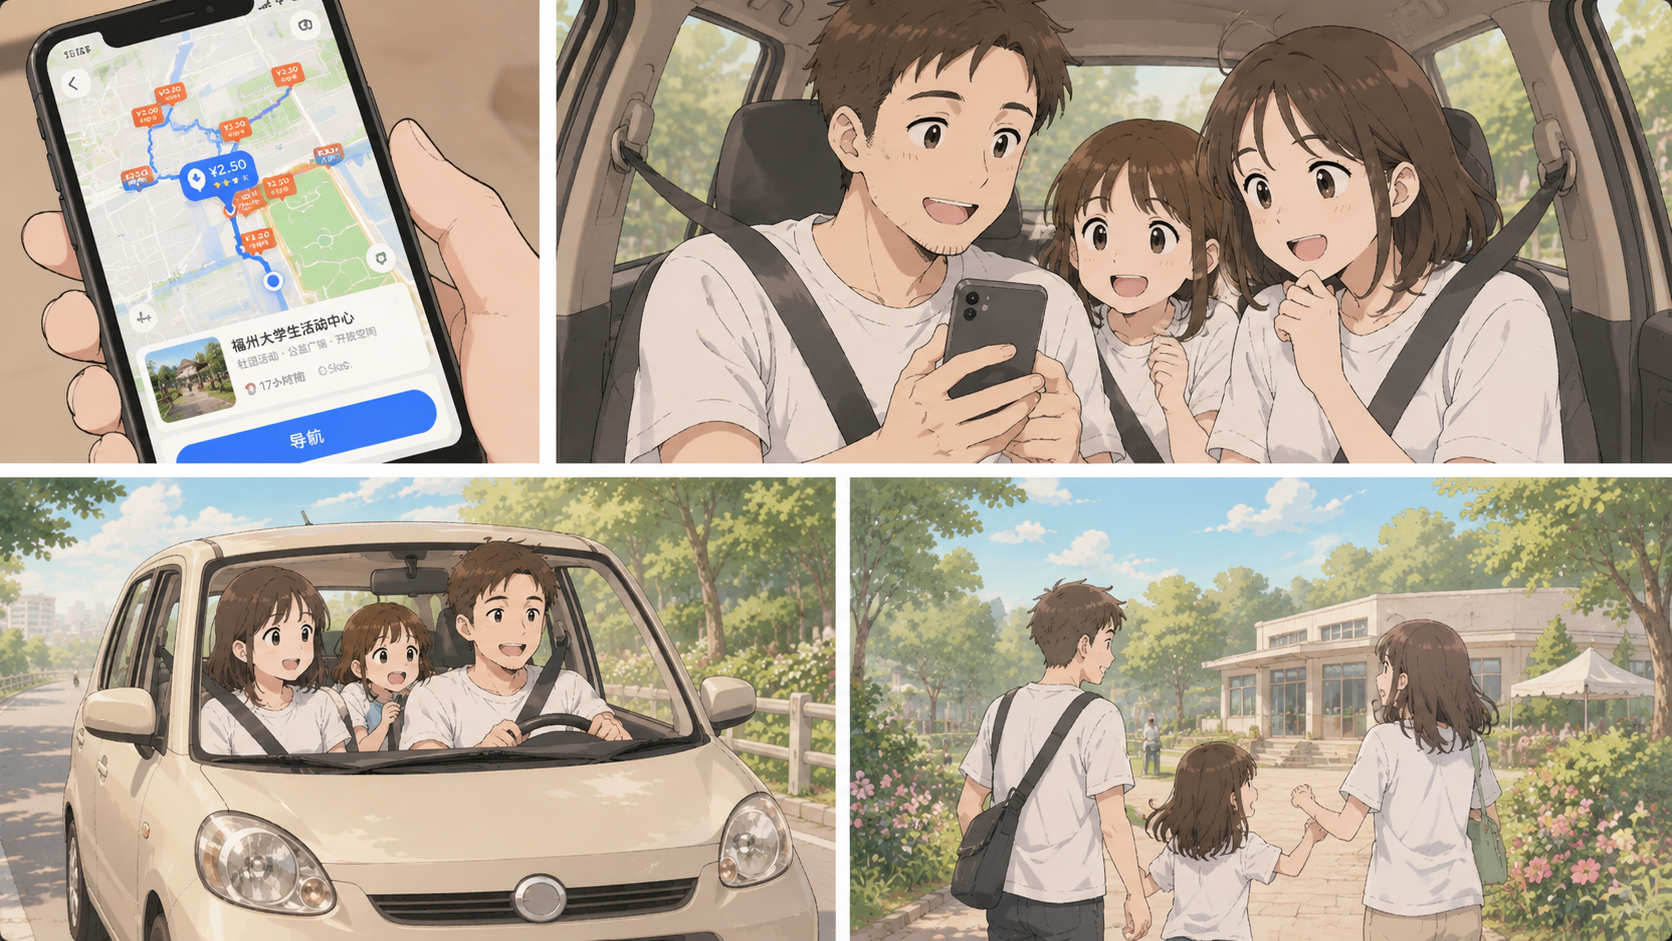
\includegraphics[width=\textwidth]{16你们决定把计划改成野餐.png}
        \caption*{决定改成野餐}
    \end{subfigure}
    \hfill
    \begin{subfigure}[b]{0.32\textwidth}
        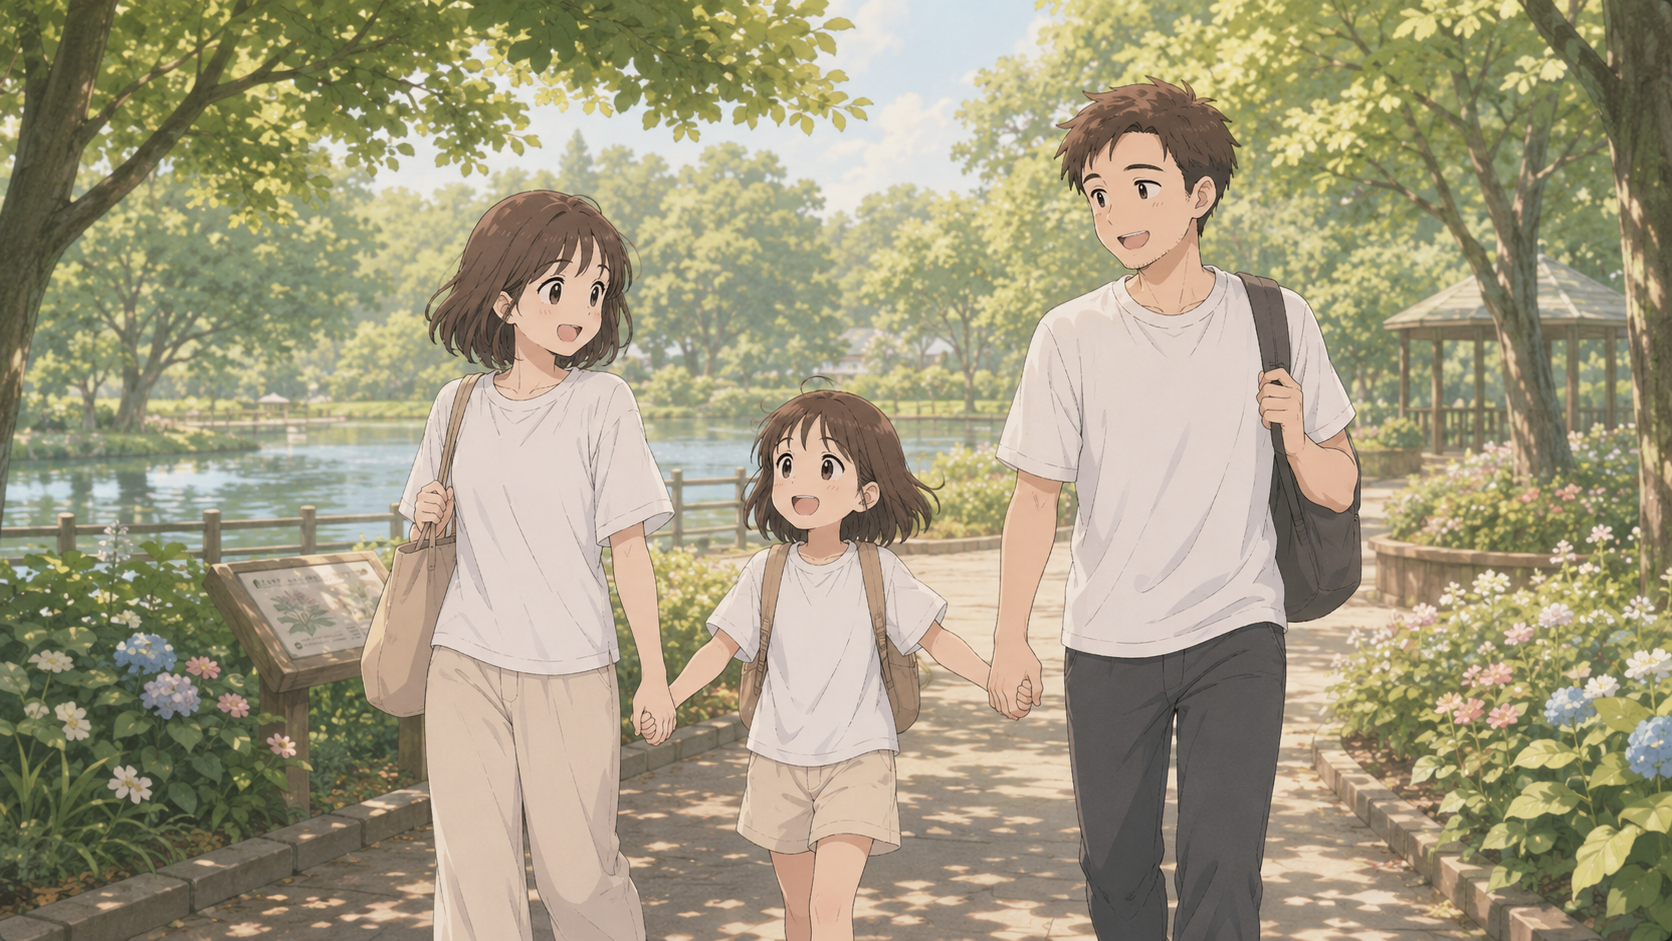
\includegraphics[width=\textwidth]{17你们把原本浪费在排队上的时间换成了春游.png}
        \caption*{享受春日时光}
    \end{subfigure}
\end{figure}

\begin{figure}[H]
    \centering
    \begin{subfigure}[b]{0.45\textwidth}
        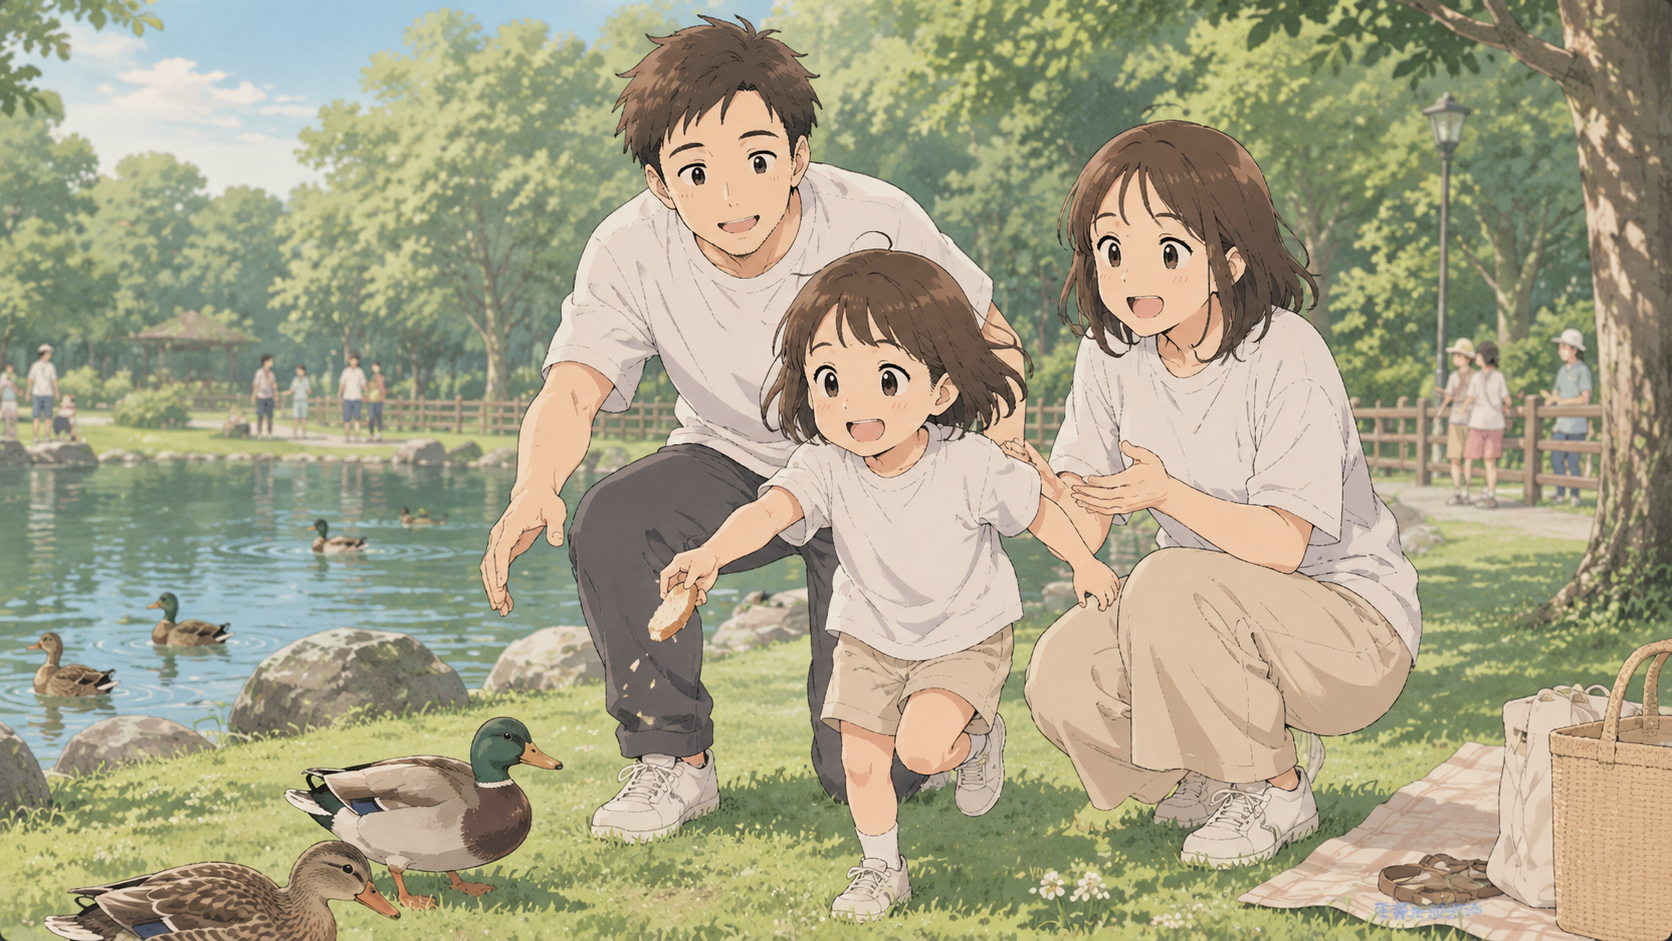
\includegraphics[width=\textwidth]{18你们玩得很开心.png}
        \caption*{一家人玩得很开心}
    \end{subfigure}
    \hfill
    \begin{subfigure}[b]{0.45\textwidth}
        
\includegraphics[width=\textwidth]{19你们一起吃冰淇淋，度过了开心的一天.png}
        \caption*{一起吃冰淇淋，开心的一天}
    \end{subfigure}
\end{figure}

\begin{center}
\fbox{\parbox{0.8\textwidth}{\centering\large
\textbf{一笔小小的悬赏}，换回了一家人的好心情，\\
省下了油钱、门票，和一个哭泣的孩子。
}}
\end{center}

\newpage

% ============================================================
%   第三章：痛点故事二 —— 酒店
% ============================================================
\section{网上的照片，你真的敢信吗？}

\begin{mdframed}[style=storystyle]
你和闺蜜计划了一次周末旅行，打开App挑酒店。

找到一家看起来不错的——宣传图精致、评分也挺高。虽然翻到几条差评说"跟图片不一样"，但好评那么多，应该没问题吧？

\vspace{6pt}
可你心里其实清楚：\textbf{很多好评是刷的}。你也想过去小红书搜搜真实评价，但打开一看——满屏都是广告和软文推广，根本分不清哪条是真的。

\vspace{6pt}
算了，宣传图确实好看，就它了。你们满怀期待地出发。
\end{mdframed}

\begin{figure}[H]
    \centering
    \begin{subfigure}[b]{0.32\textwidth}
        
\includegraphics[width=\textwidth]{21两个女孩一起选酒店.png}
        \caption*{和闺蜜一起选酒店}
    \end{subfigure}
    \hfill
    \begin{subfigure}[b]{0.32\textwidth}
        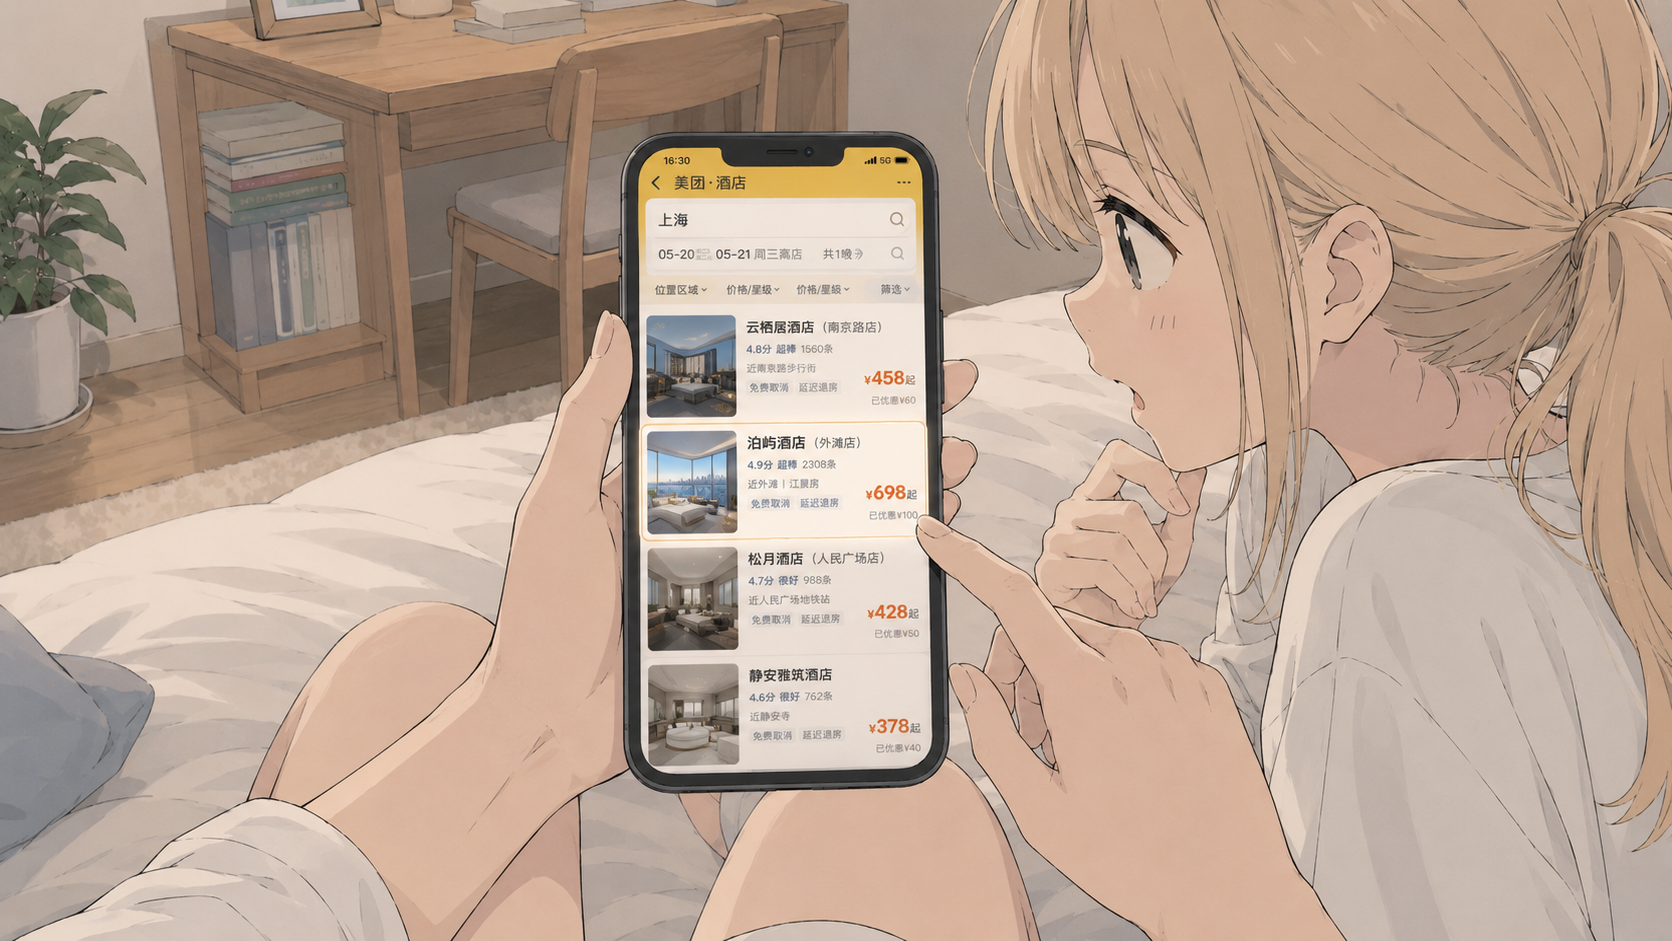
\includegraphics[width=\textwidth]{22你们找到了酒店.png}
        \caption*{找到了一家酒店}
    \end{subfigure}
    \hfill
    \begin{subfigure}[b]{0.32\textwidth}
        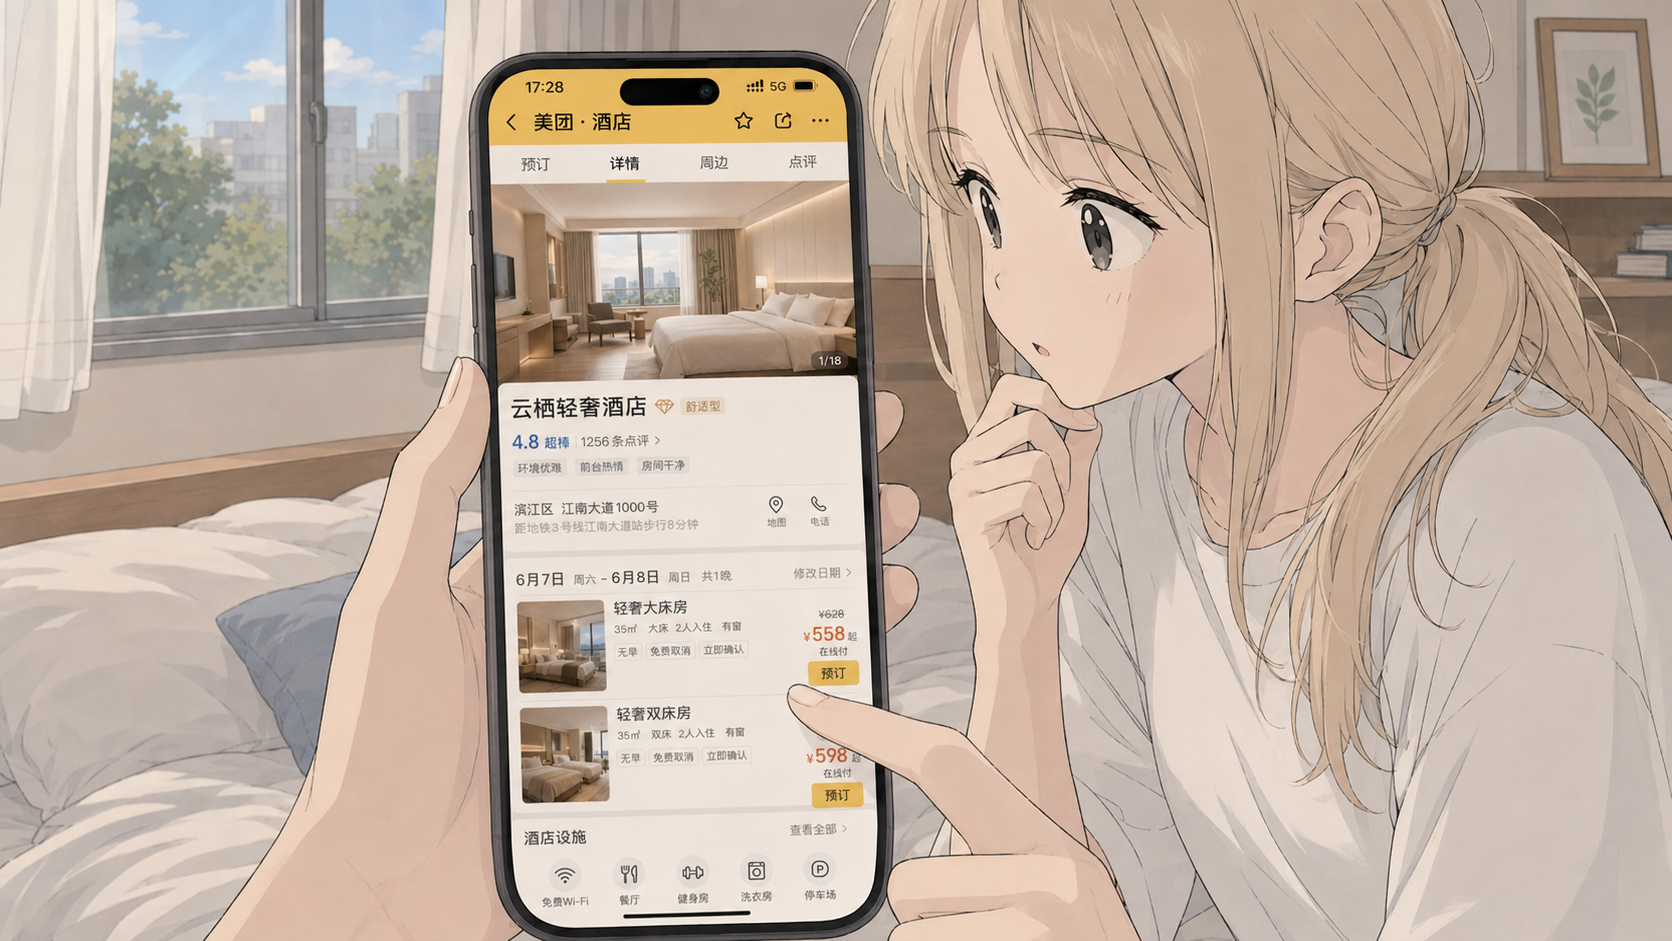
\includegraphics[width=\textwidth]{23看宣传图还不错.png}
        \caption*{宣传图看着还不错}
    \end{subfigure}
\end{figure}

\begin{figure}[H]
    \centering
    \begin{subfigure}[b]{0.32\textwidth}
        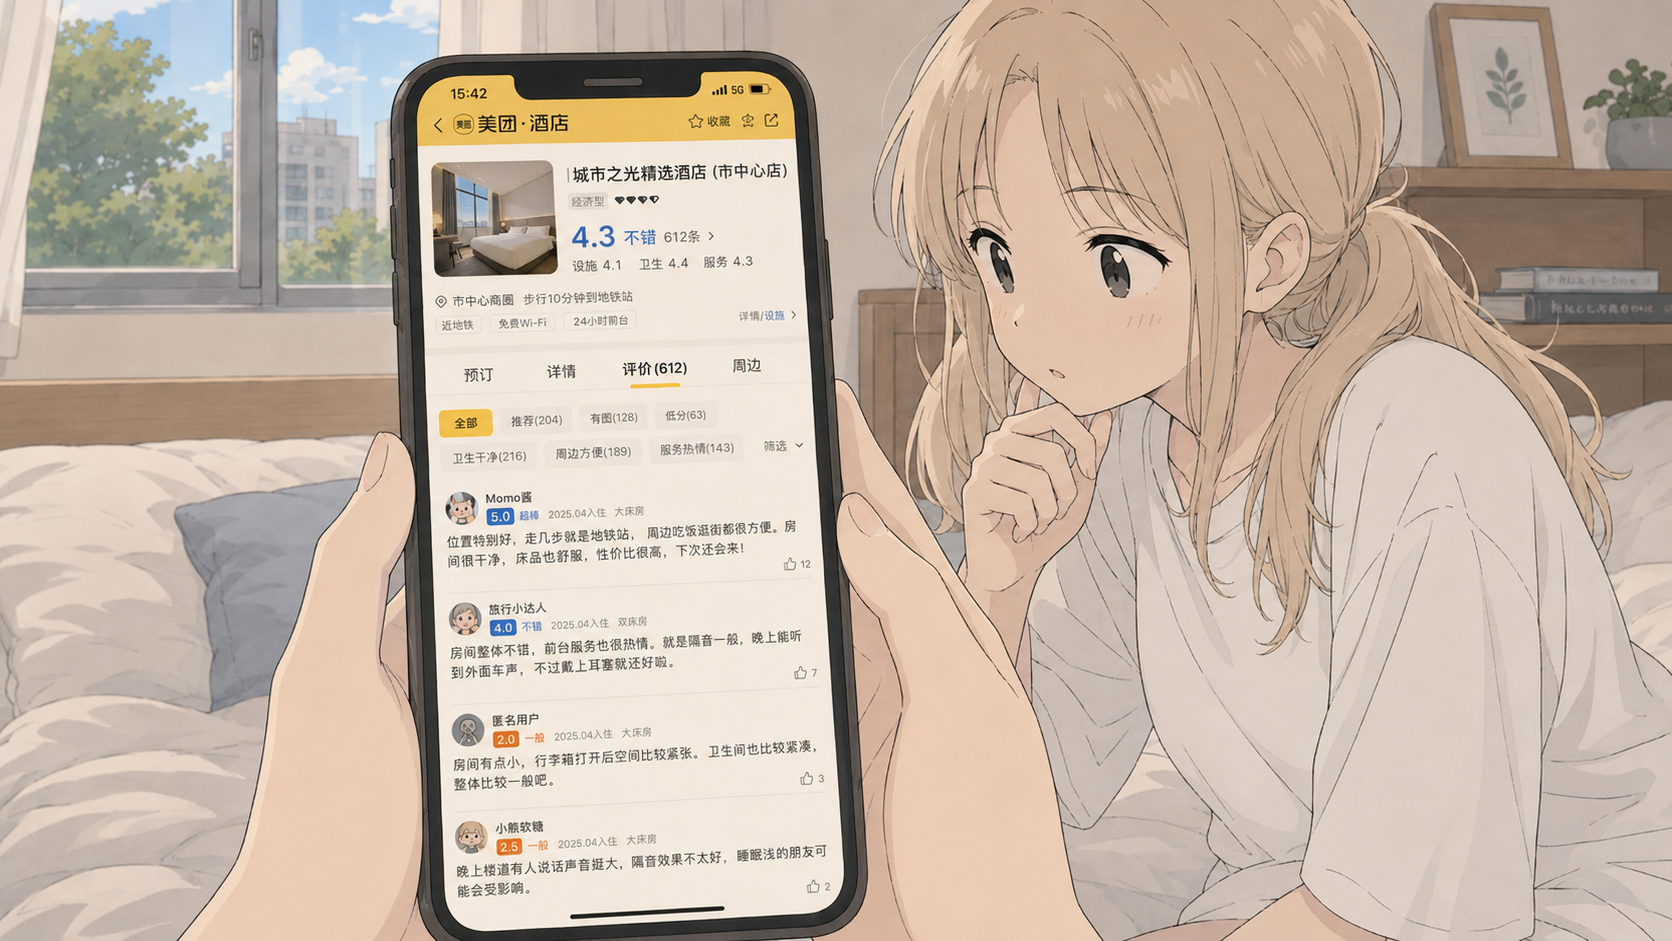
\includegraphics[width=\textwidth]{24评论看上去也还行.png}
        \caption*{评论看上去也还行}
    \end{subfigure}
    \hfill
    \begin{subfigure}[b]{0.32\textwidth}
        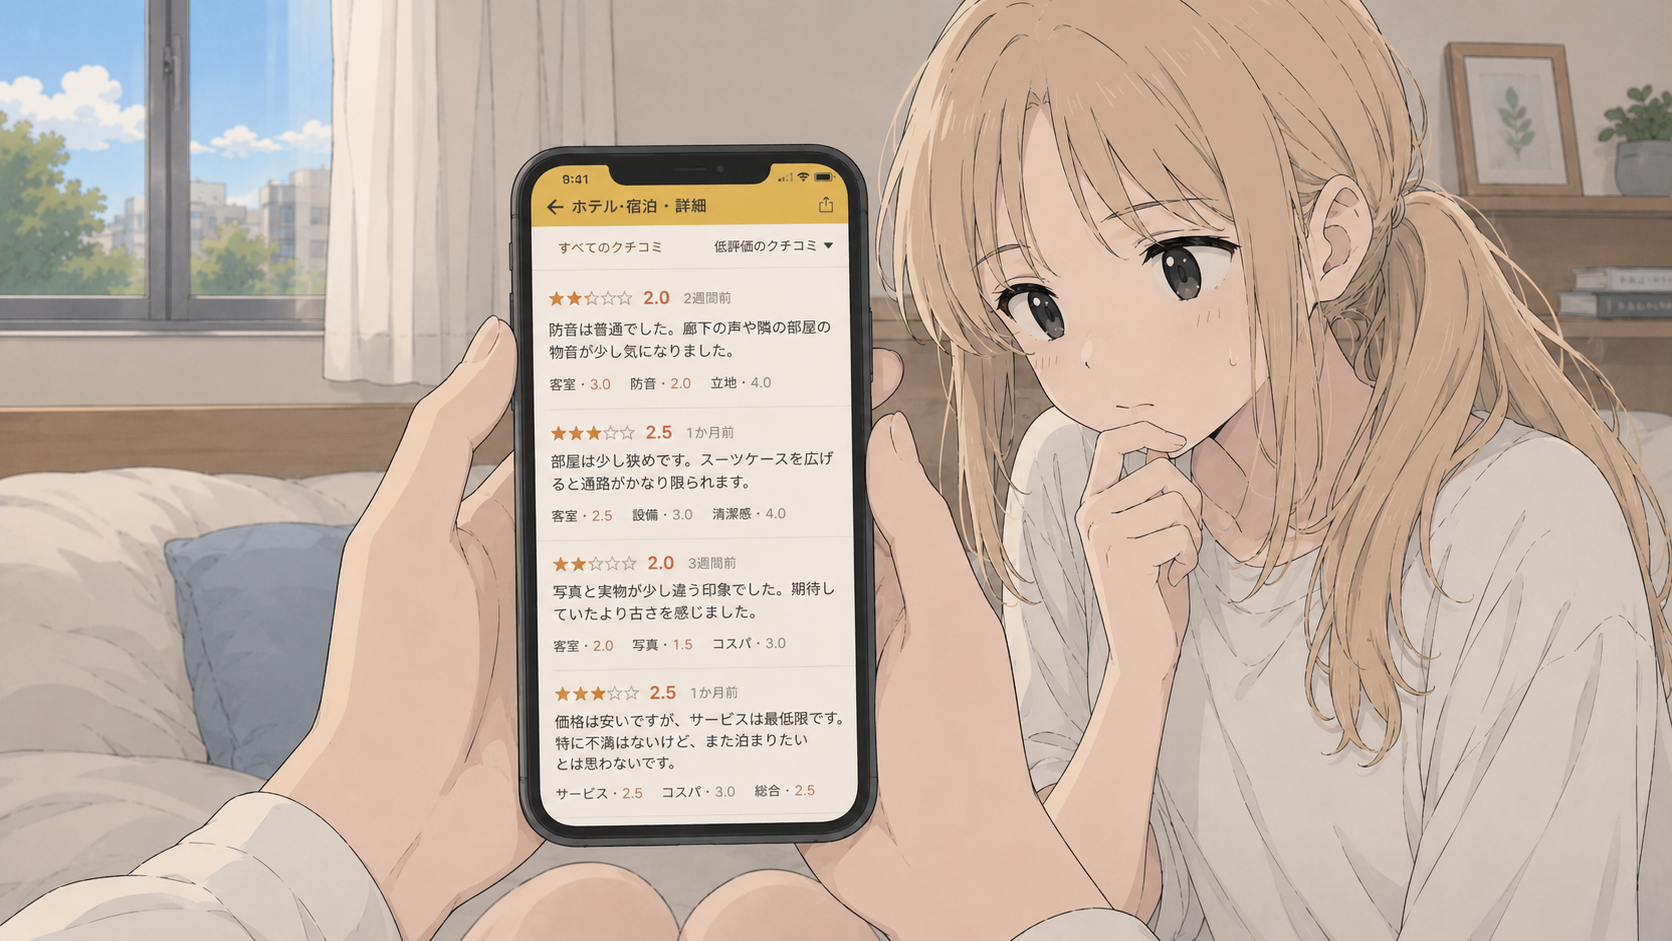
\includegraphics[width=\textwidth]{25有些差评，但是你还是决定试试.png}
        \caption*{有差评，但决定试试}
    \end{subfigure}
    \hfill
    \begin{subfigure}[b]{0.32\textwidth}
        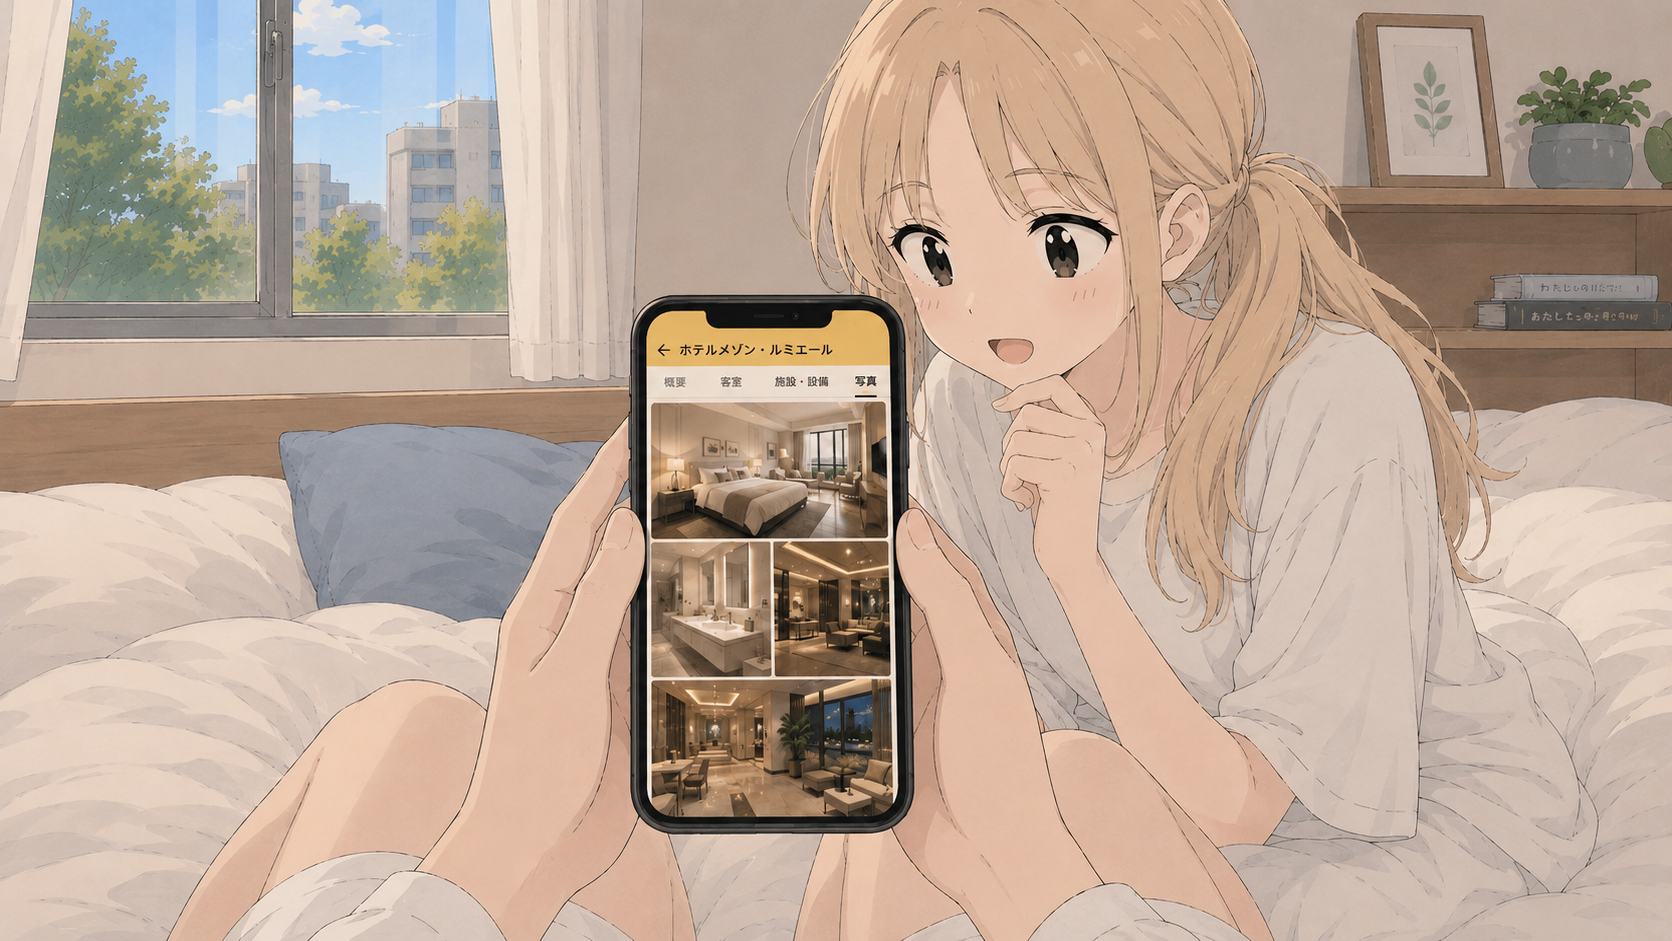
\includegraphics[width=\textwidth]{26因为你看到了宣传图，感觉很不错.png}
        \caption*{宣传图实在太吸引人}
    \end{subfigure}
\end{figure}

{\color{painred}\bfseries \large 到了之后……}
\begin{mdframed}[style=painstyle]
你们兴冲冲地到了酒店，迫不及待打开房门——

结果眼前的景象和宣传图\textbf{完全不一样}。房间比想象中小很多，装修陈旧，灯光昏暗，跟精心修图的宣传照简直是两个地方。

\vspace{6pt}
退房？钱已经付了，不给退。忍着住？一整晚都别扭。

\vspace{6pt}
你们面面相觑，旅行的好心情瞬间跌到谷底。

\textbf{其实那几条差评说的都是真的，只是被刷出来的好评淹没了。}
\end{mdframed}

\begin{figure}[H]
    \centering
    \begin{subfigure}[b]{0.32\textwidth}
        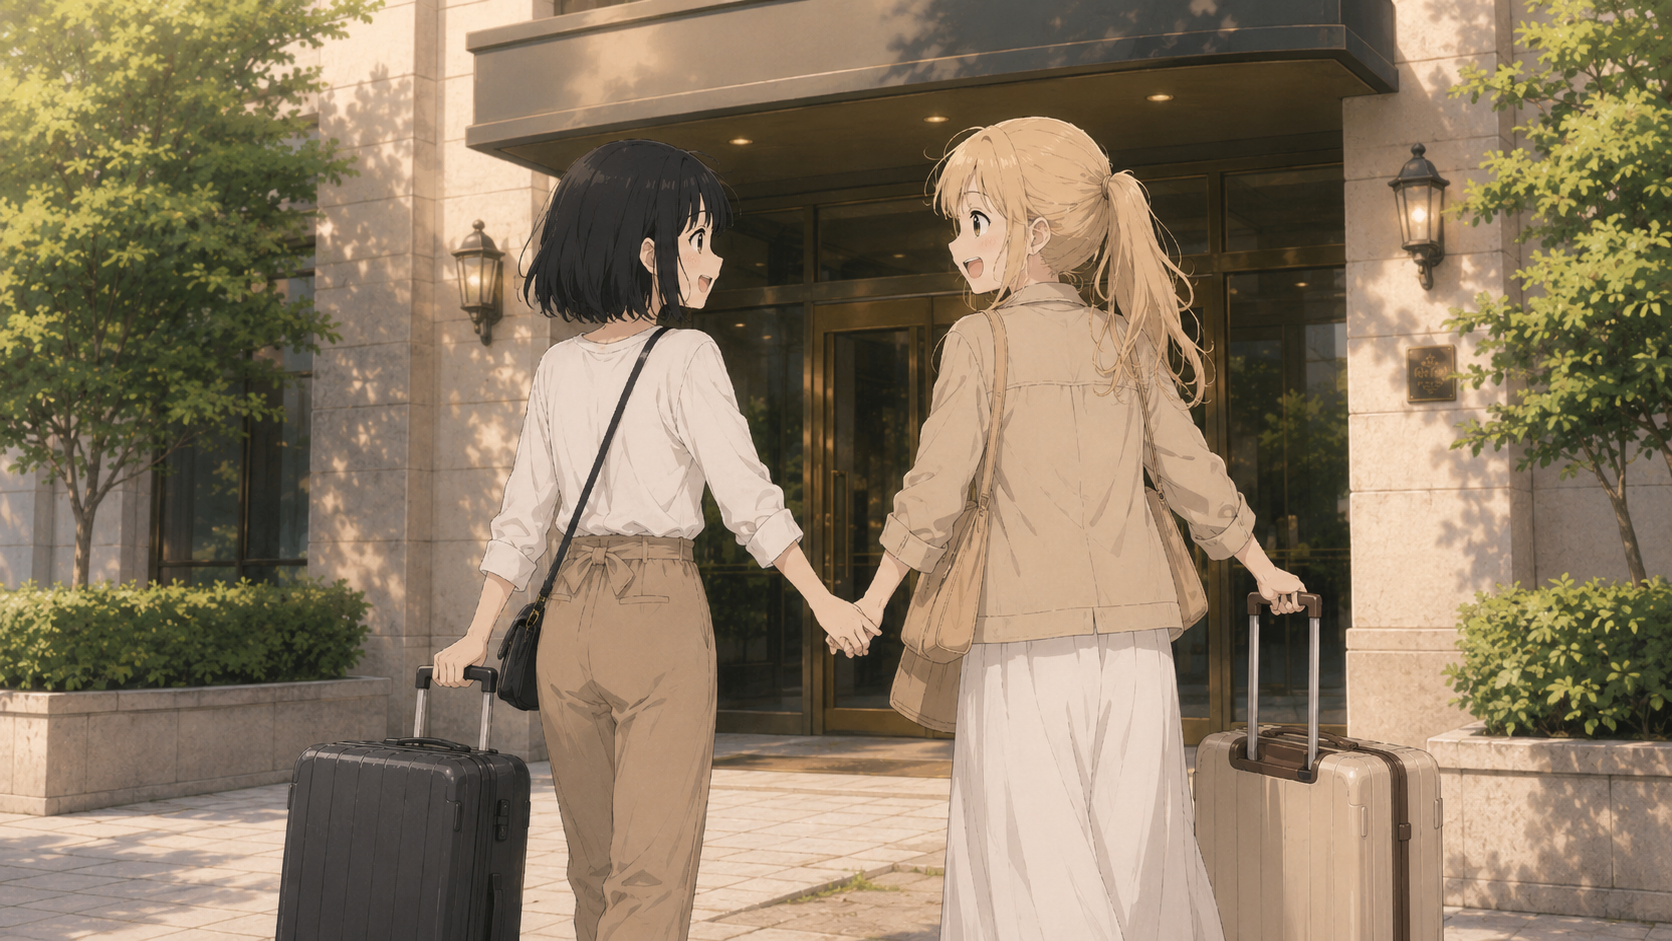
\includegraphics[width=\textwidth]{27你和闺蜜一起去了酒店.png}
        \caption*{和闺蜜一起到了酒店}
    \end{subfigure}
    \hfill
    \begin{subfigure}[b]{0.32\textwidth}
        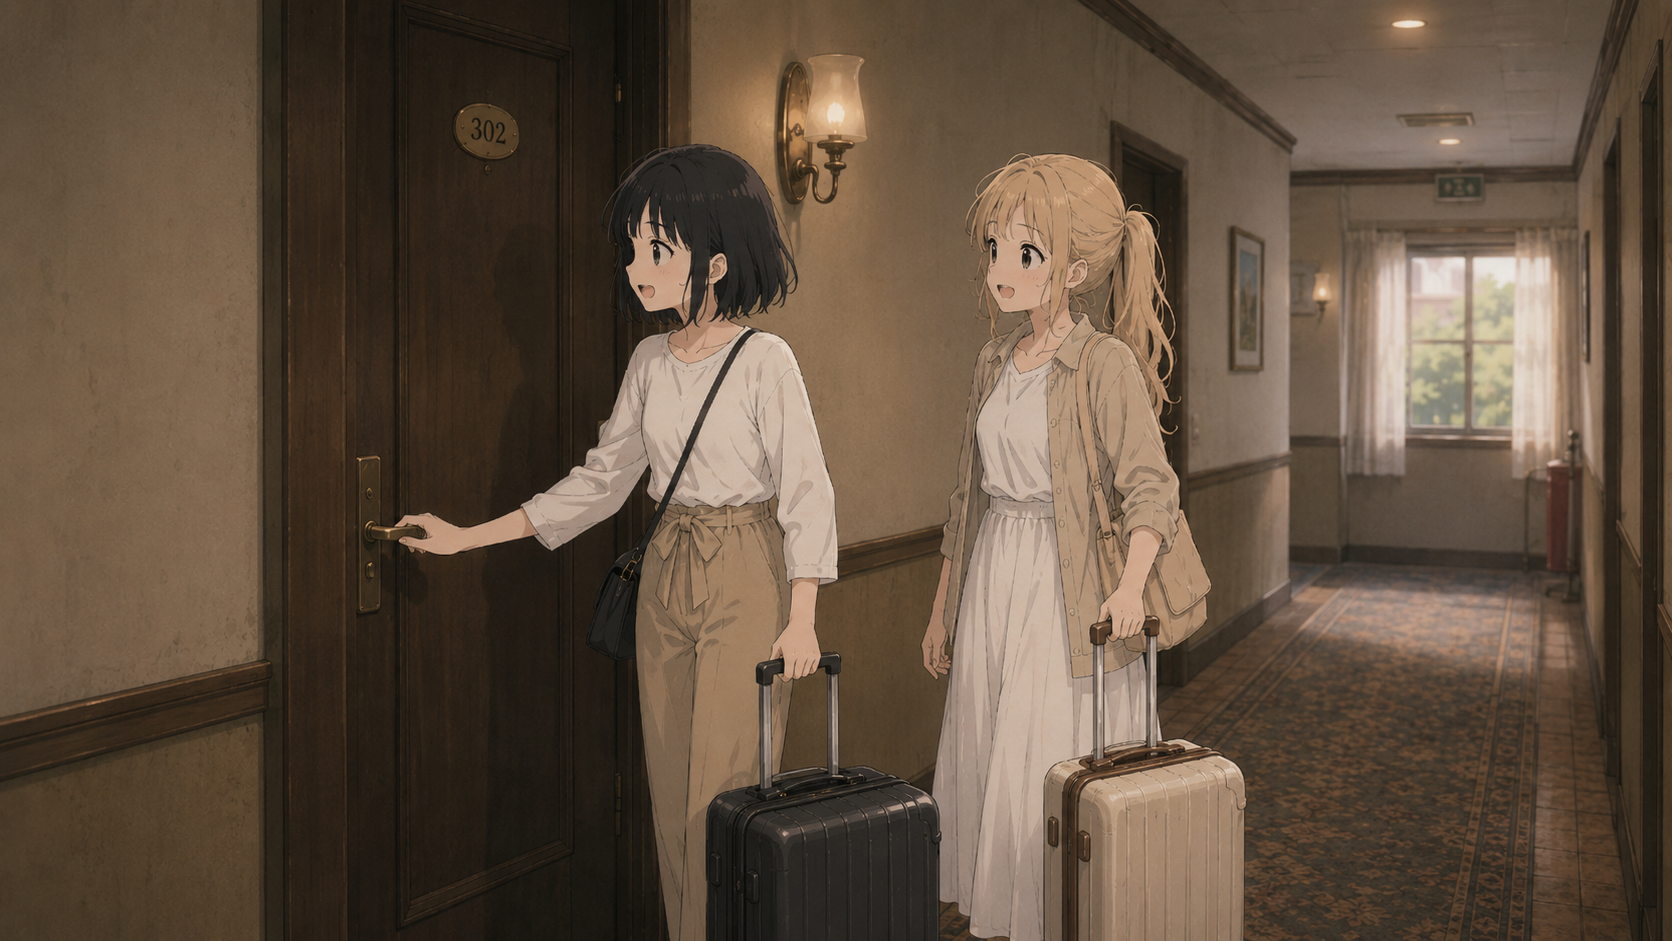
\includegraphics[width=\textwidth]{28你们迫不及待打开门.png}
        \caption*{迫不及待打开门}
    \end{subfigure}
    \hfill
    \begin{subfigure}[b]{0.32\textwidth}
        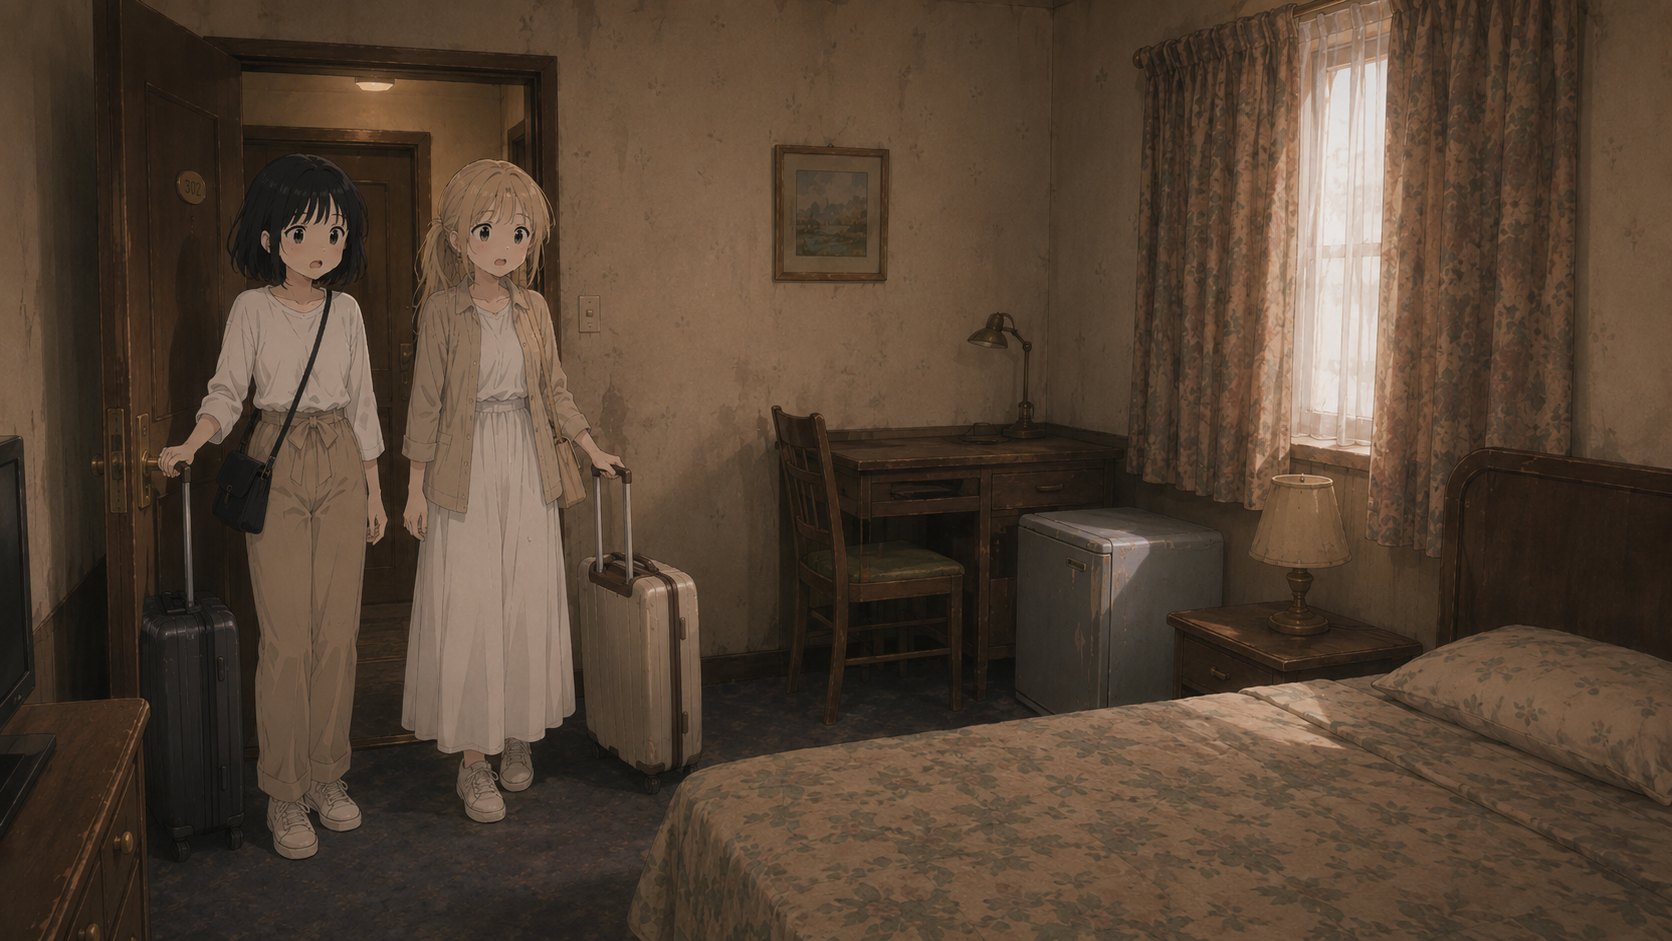
\includegraphics[width=\textwidth]{29结果酒店的真实情况跟宣传图相差很大.png}
        \caption*{现实与宣传图相差甚远}
    \end{subfigure}
\end{figure}

\begin{figure}[H]
    \centering
    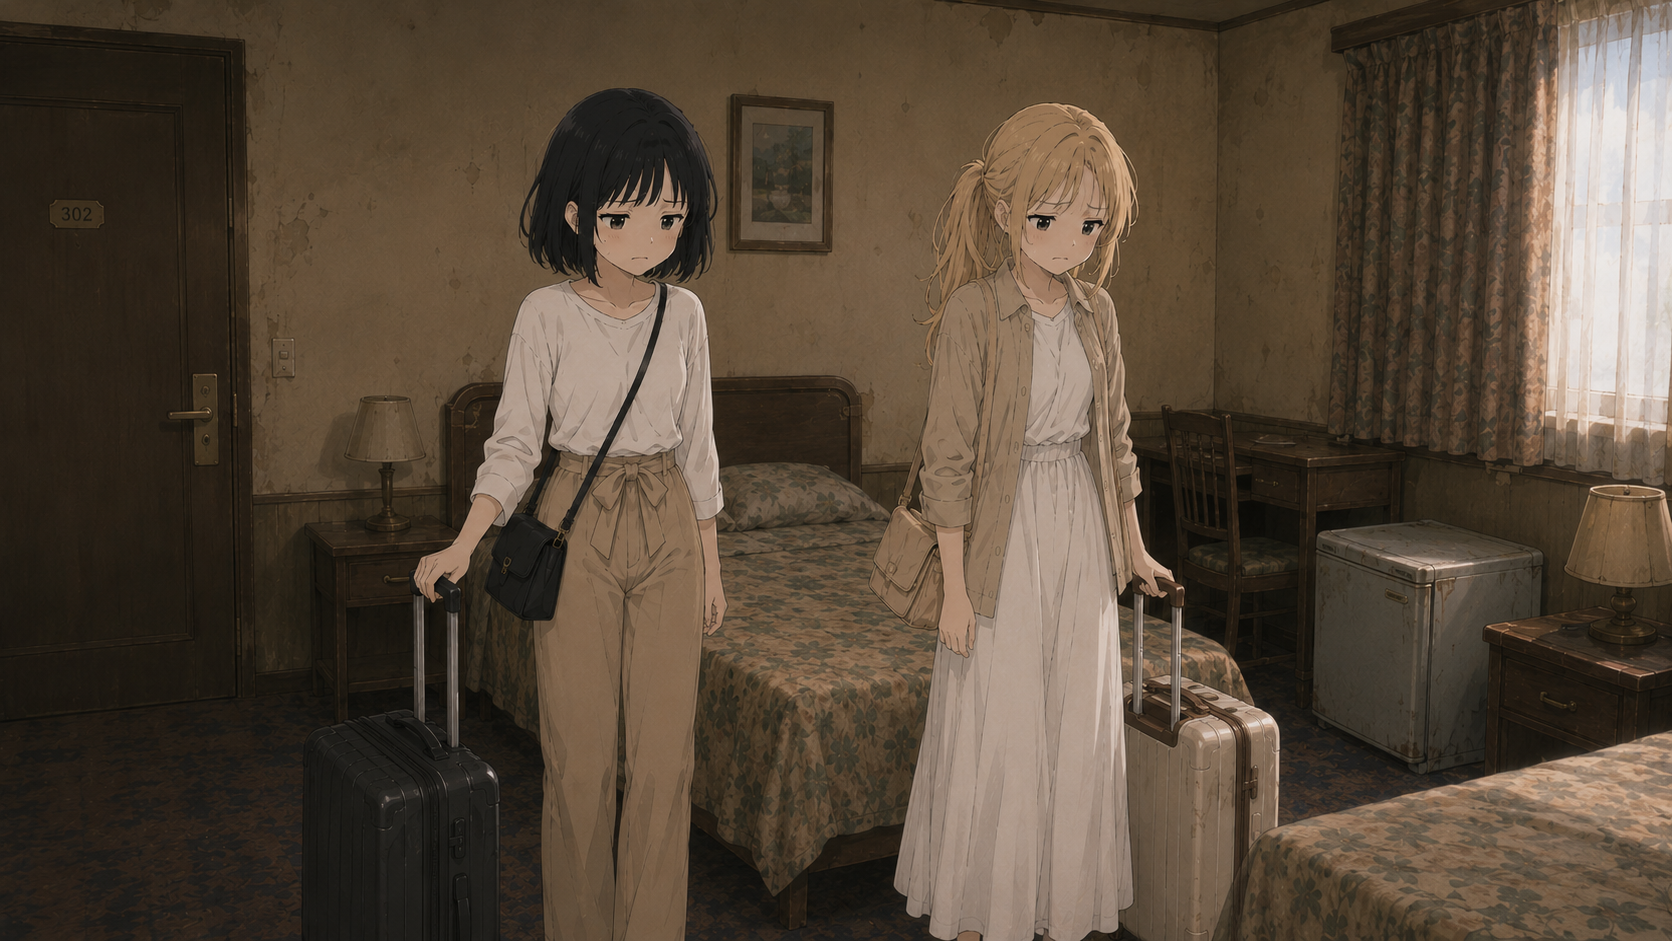
\includegraphics[width=0.4\textwidth]{30你们觉得很失落.png}
    \caption*{\small 满心期待变成满心失落}
\end{figure}

\vspace{0.3cm}

{\color{hopegreen}\bfseries \large 如果你提前用了「实时探路」呢？}
\begin{mdframed}[style=hopestyle]
订房之前，你发布了一个任务：

\begin{center}
\itshape "有没有人刚好住在XX酒店？帮我拍一下房间真实环境，跟宣传图差别大吗？"
\end{center}

\vspace{4pt}
刚好有一位在美团订了同一家酒店的住客看到了你的任务。他随手拍了几张真实的照片发给你——房间实景、窗外环境、走廊灯光，所见即所得。

\vspace{6pt}
\textbf{跟小红书和平台评论不同}，实时探路通过GPS定位验证，确保回答者\textbf{真的在那个地方}。不是广告，不是软文，不是几个月前的过期信息——就是此时此刻的真实情况。

\vspace{6pt}
你提前避开了这个坑，换了一家真正靠谱的酒店。闺蜜旅行，从第一步就是对的。
\end{mdframed}

\newpage

% ============================================================
%   第四章：产品介绍
% ============================================================
\section{实时探路是什么？}

\textbf{实时探路}是一个基于位置的实时信息众包平台。

它连接两类人：
\begin{itemize}[leftmargin=2em]
    \item \textbf{想了解某地实况的人}（发布者）——出发前想知道目的地真实情况
    \item \textbf{正在该地附近的人}（接单者）——顺手拍几张照片就能赚零花钱
\end{itemize}

\vspace{0.3cm}

\begin{mdframed}[style=infostyle]
\textbf{一句话概括：}花几块钱，让已经在那里的人帮你看一眼。

\vspace{6pt}
跟刷评论、看小红书、问朋友不同——实时探路通过\textbf{GPS定位}保证回答者确实在现场，你看到的就是\textbf{此时此刻}的真实状况。
\end{mdframed}

\subsection{适用场景}

\begin{table}[H]
\centering
\renewcommand{\arraystretch}{1.4}
\begin{tabularx}{\textwidth}{>{\bfseries}l X l}
\toprule
场景 & 痛点 & 价值 \\
\midrule
景点出游 & 到了才发现人山人海，假期白费 & 提前知道拥挤程度 \\
网红餐厅 & 专程跑一趟发现排队2小时或售罄 & 实时排队情况 \\
商场/展览 & 不确定是否值得去 & 现场照片辅助决策 \\
酒店民宿 & 宣传图美化、好评是刷的 & 真实环境验证 \\
\bottomrule
\end{tabularx}
\end{table}

\newpage

% ============================================================
%   第五章：核心功能
% ============================================================
\section{核心功能}

\subsection{发布任务}

\begin{itemize}[leftmargin=2em]
    \item 选择目标地点（地图选点/搜索地址）
    \item 描述你想了解的内容（排队情况、某商品是否有货、环境等）
    \item 设置悬赏金额（最低0.01元起）
    \item 设置任务有效期（30分钟 / 1小时 / 2小时 / 4小时 / 12小时 / 24小时）
    \item 指定需要的照片数量
    \item 可附加拍摄要求（如"拍门口排队情况"、"拍菜单价格"）
\end{itemize}

\subsection{接单与提交}

\begin{itemize}[leftmargin=2em]
    \item 浏览附近的悬赏任务（默认5公里搜索范围）
    \item 接单时需在任务地点\textbf{1000米}范围内（GPS定位校验）
    \item 提交时同样需在任务地点\textbf{1000米}范围内
    \item 提交内容：现场照片（按要求数量）+ 文字描述
    \item 支持实时聊天：发布者可以追加问题，接单者实时回复
\end{itemize}

\subsection{确认与支付}

\begin{itemize}[leftmargin=2em]
    \item 发布者收到提交通知，查看照片和描述
    \item 满意 → 确认收货，悬赏金自动发放给接单者
    \item 不满意 → 拒绝并说明原因，接单者可重新提交
    \item 超时未操作 → 24小时后自动确认支付（保护接单者权益）
    \item 接单者也可主动放弃任务，任务重新开放
\end{itemize}

\subsection{信用与评价}

\begin{itemize}[leftmargin=2em]
    \item 任务完成后双方互评（1-5星 + 文字评价）
    \item 贝叶斯均值评分系统（基准5.0分，避免少量评价极端波动）
    \item 历史完成记录公开可查
\end{itemize}

\newpage

% ============================================================
%   第六章：产品界面
% ============================================================
\section{产品界面展示}

\begin{figure}[H]
    \centering
    \begin{subfigure}[b]{0.3\textwidth}
        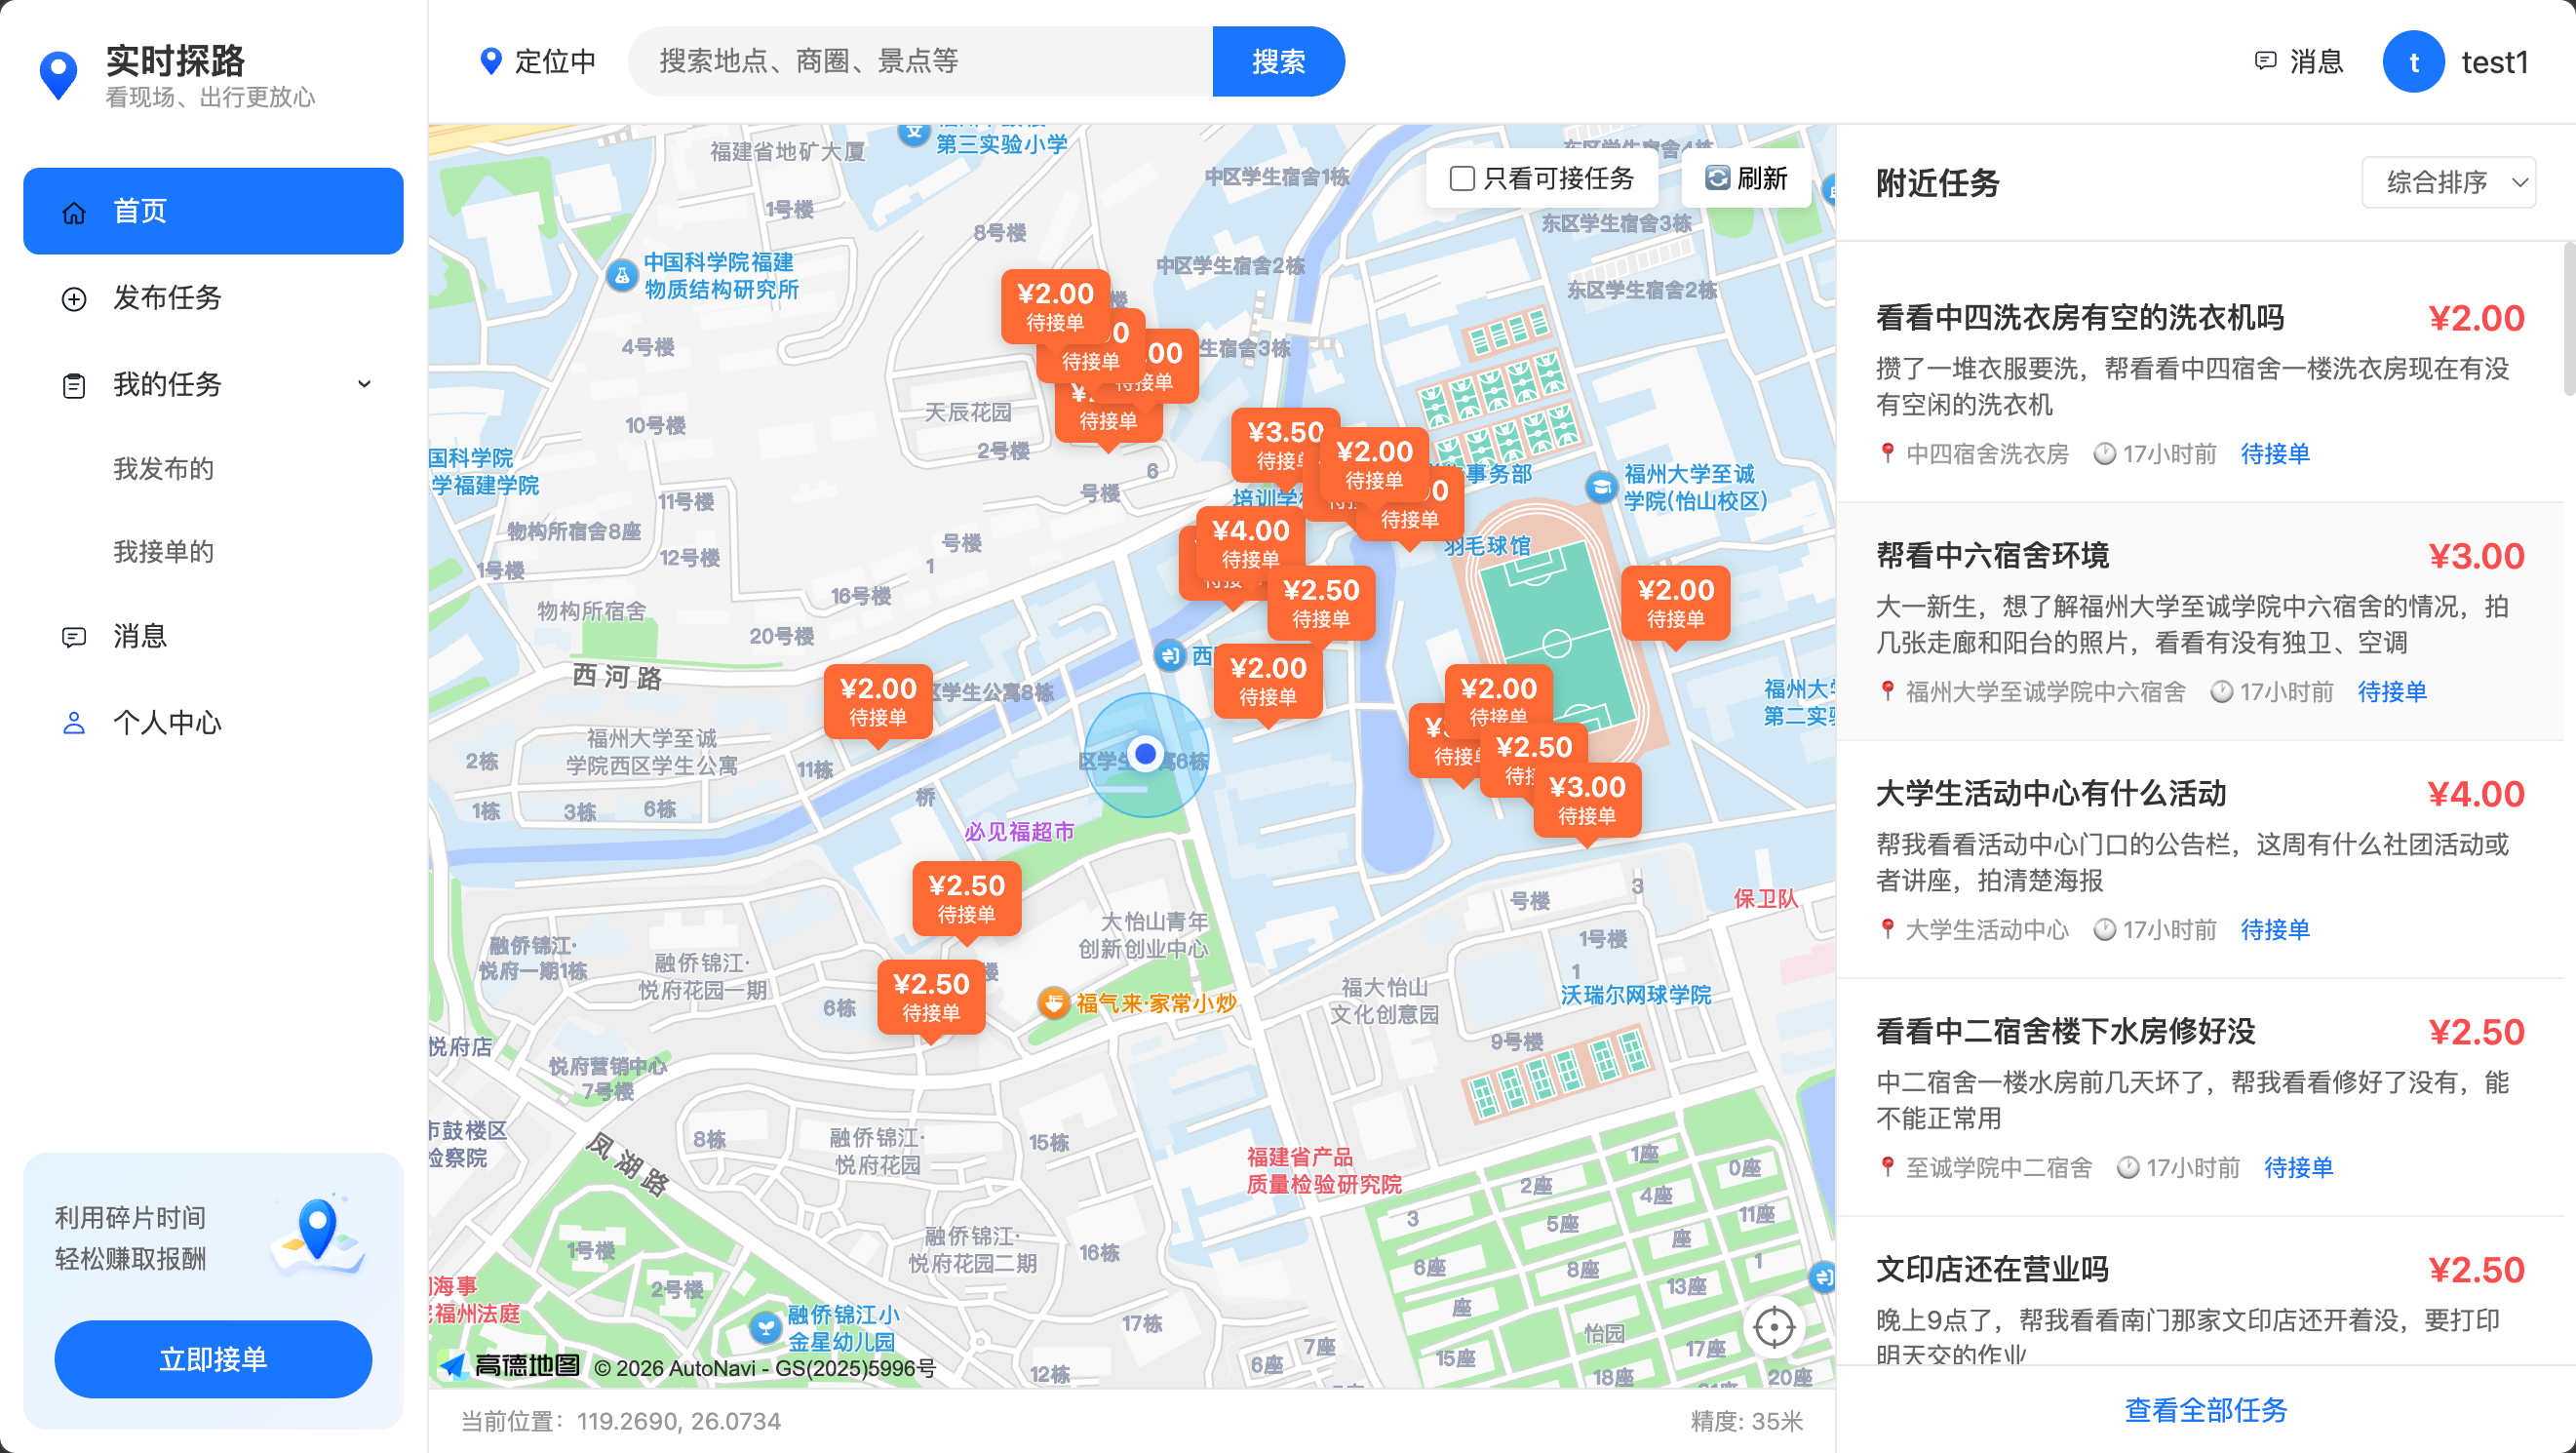
\includegraphics[width=\textwidth]{首页.png}
        \caption*{\small 首页：地图展示附近任务}
    \end{subfigure}
    \hfill
    \begin{subfigure}[b]{0.3\textwidth}
        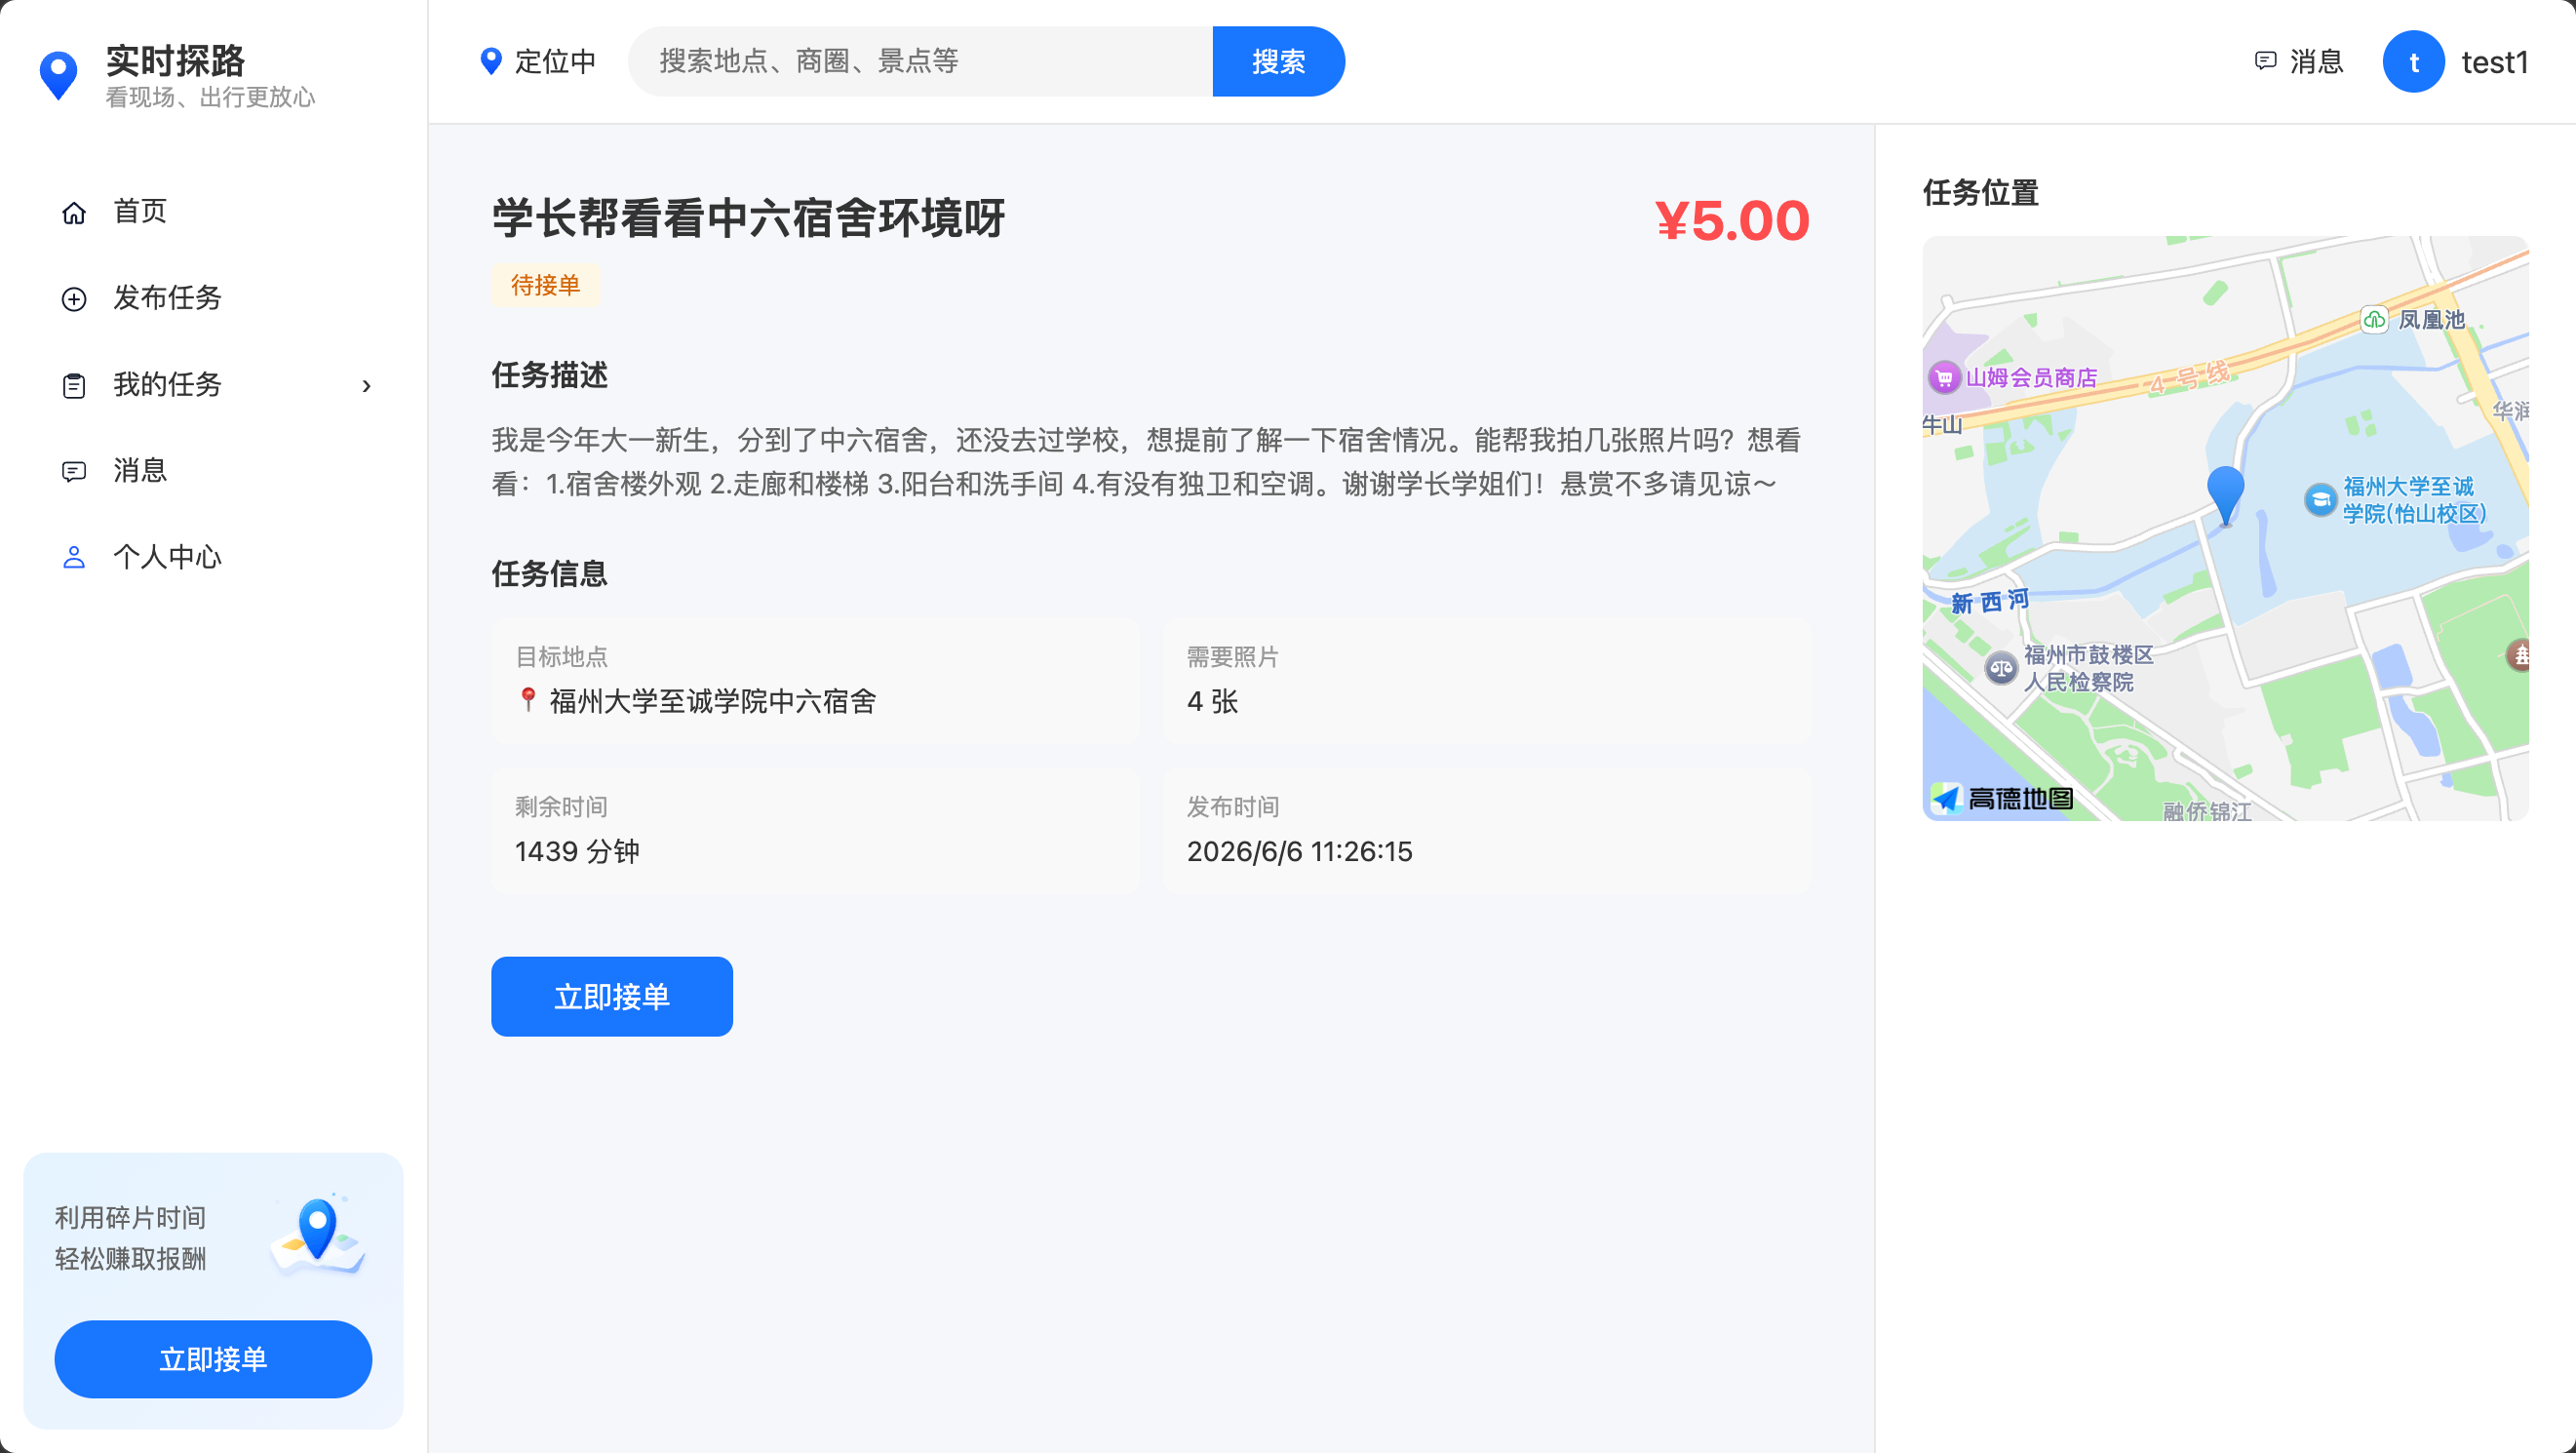
\includegraphics[width=\textwidth]{接单.png}
        \caption*{\small 接单页：浏览可接任务}
    \end{subfigure}
    \hfill
    \begin{subfigure}[b]{0.3\textwidth}
        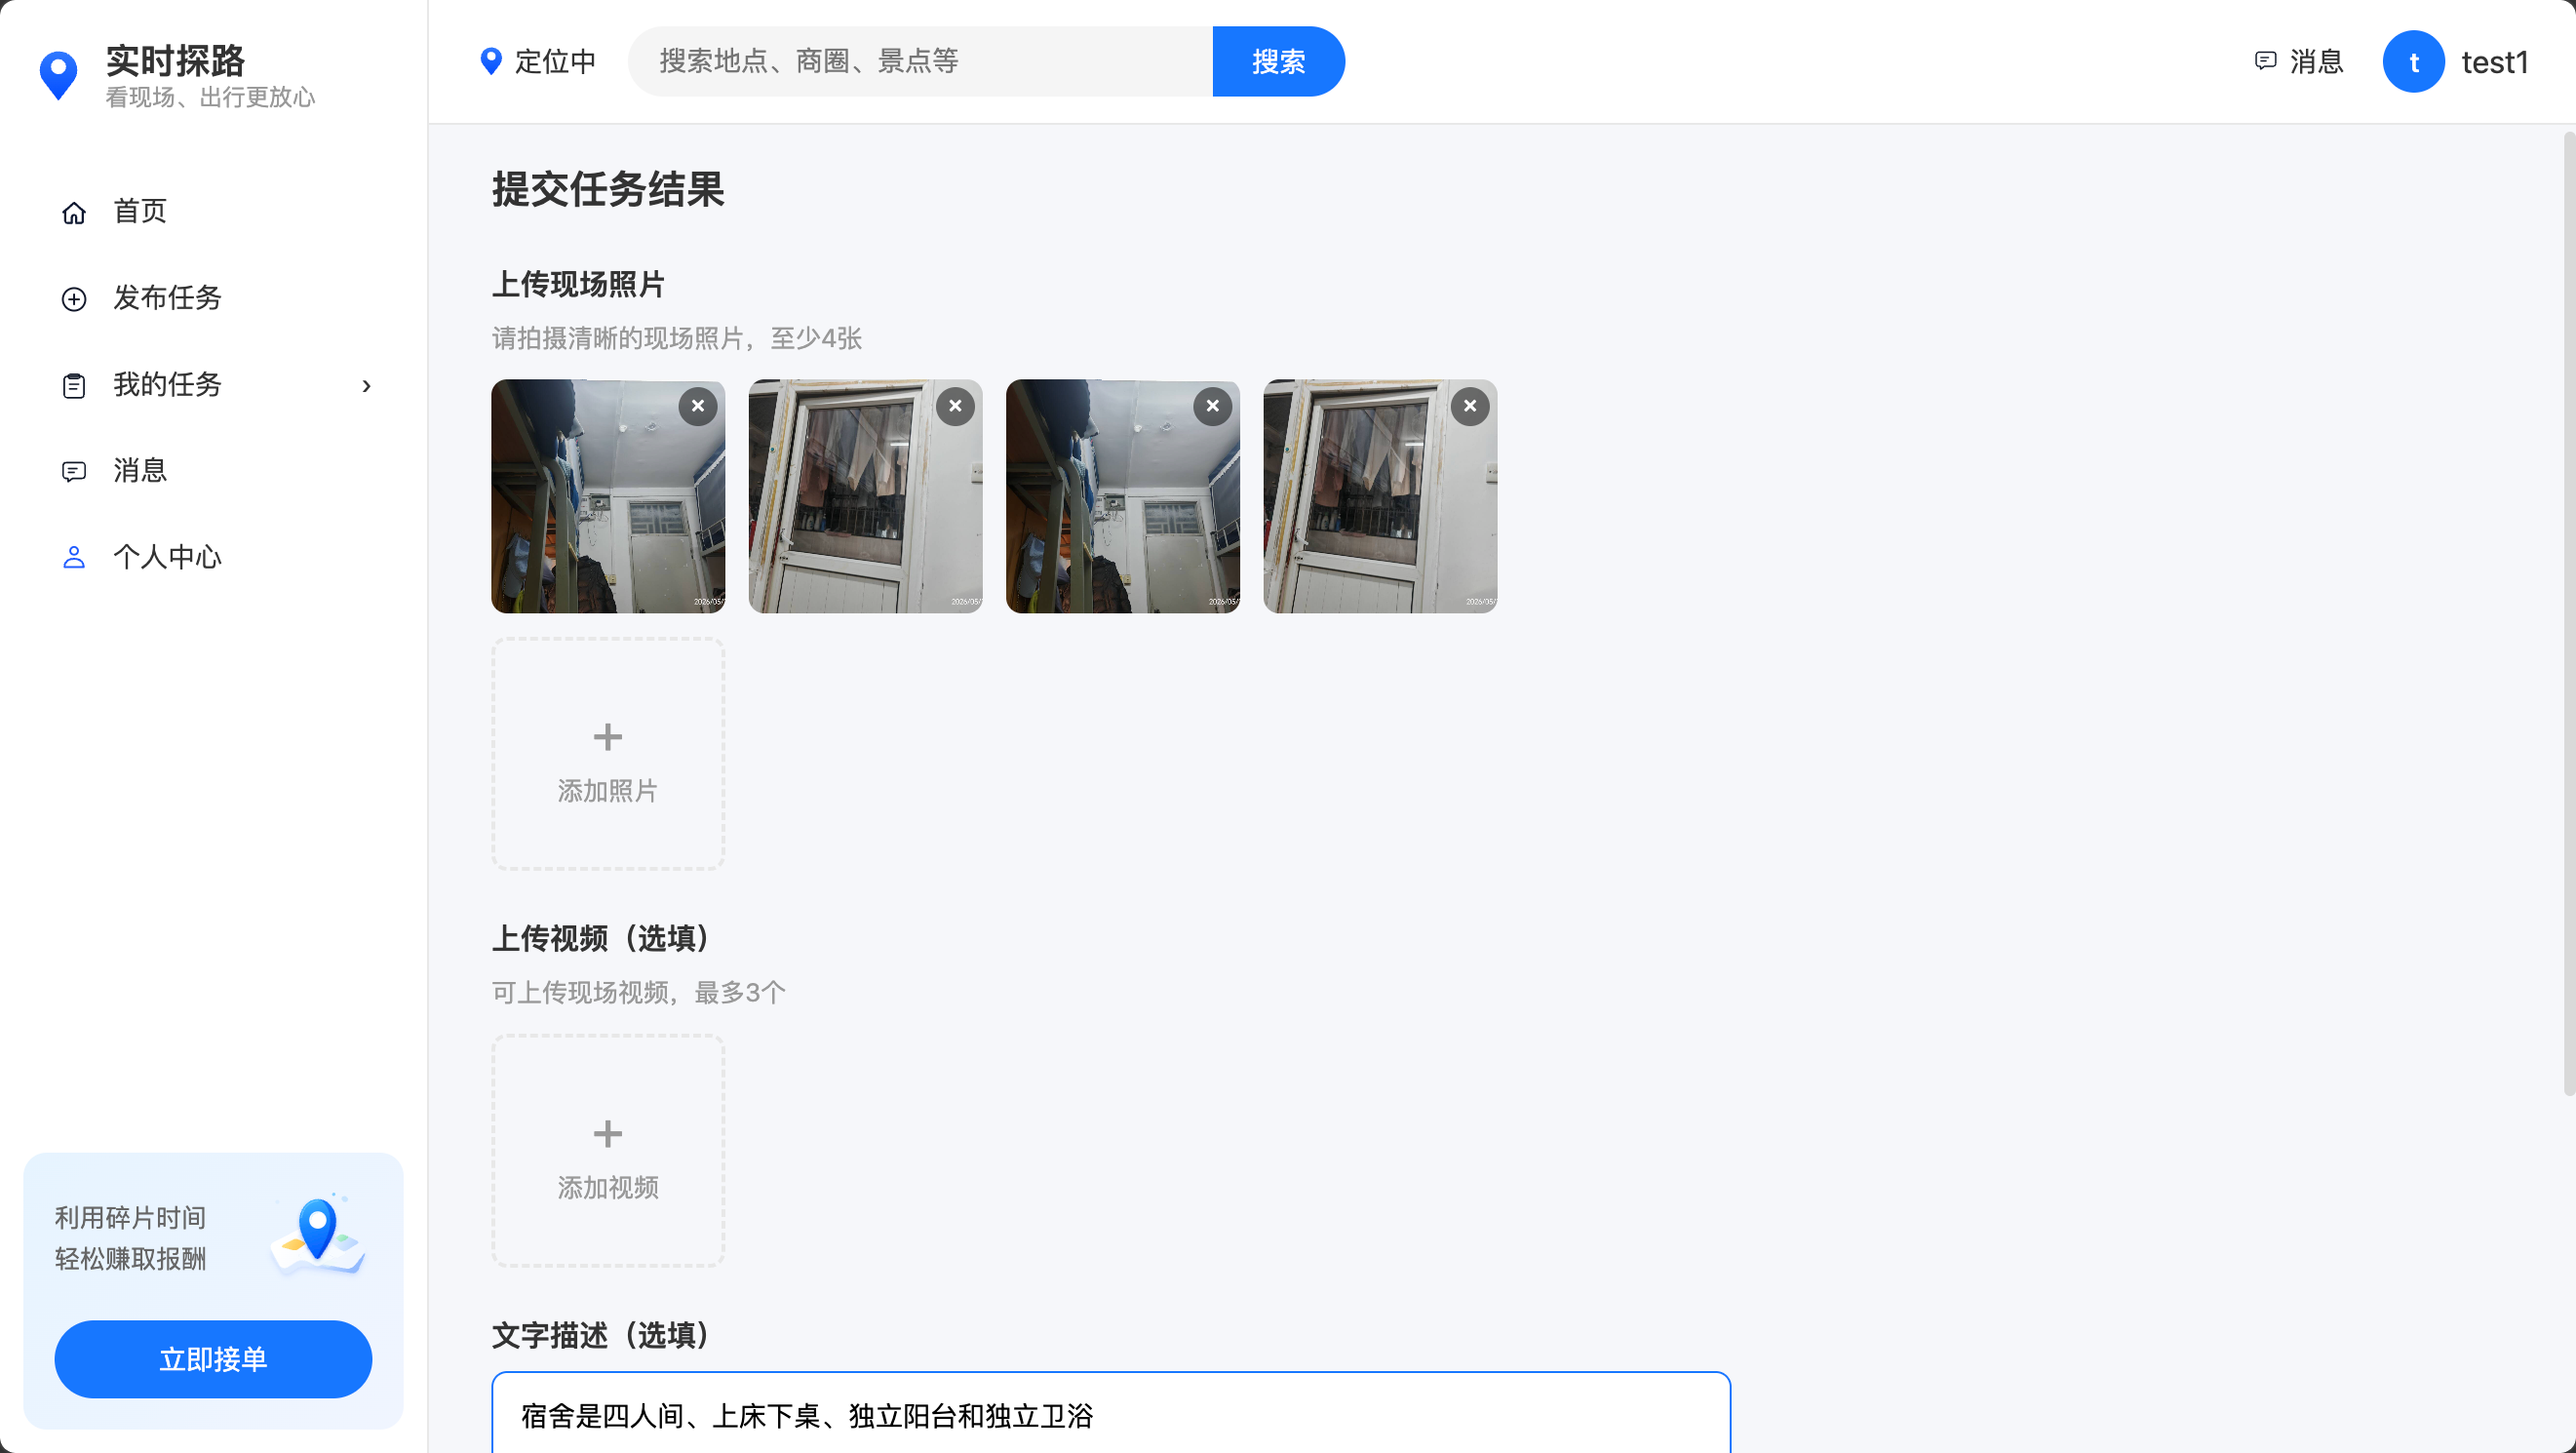
\includegraphics[width=\textwidth]{提交任务.png}
        \caption*{\small 提交：拍照+描述现场情况}
    \end{subfigure}
\end{figure}

\begin{figure}[H]
    \centering
    \begin{subfigure}[b]{0.4\textwidth}
        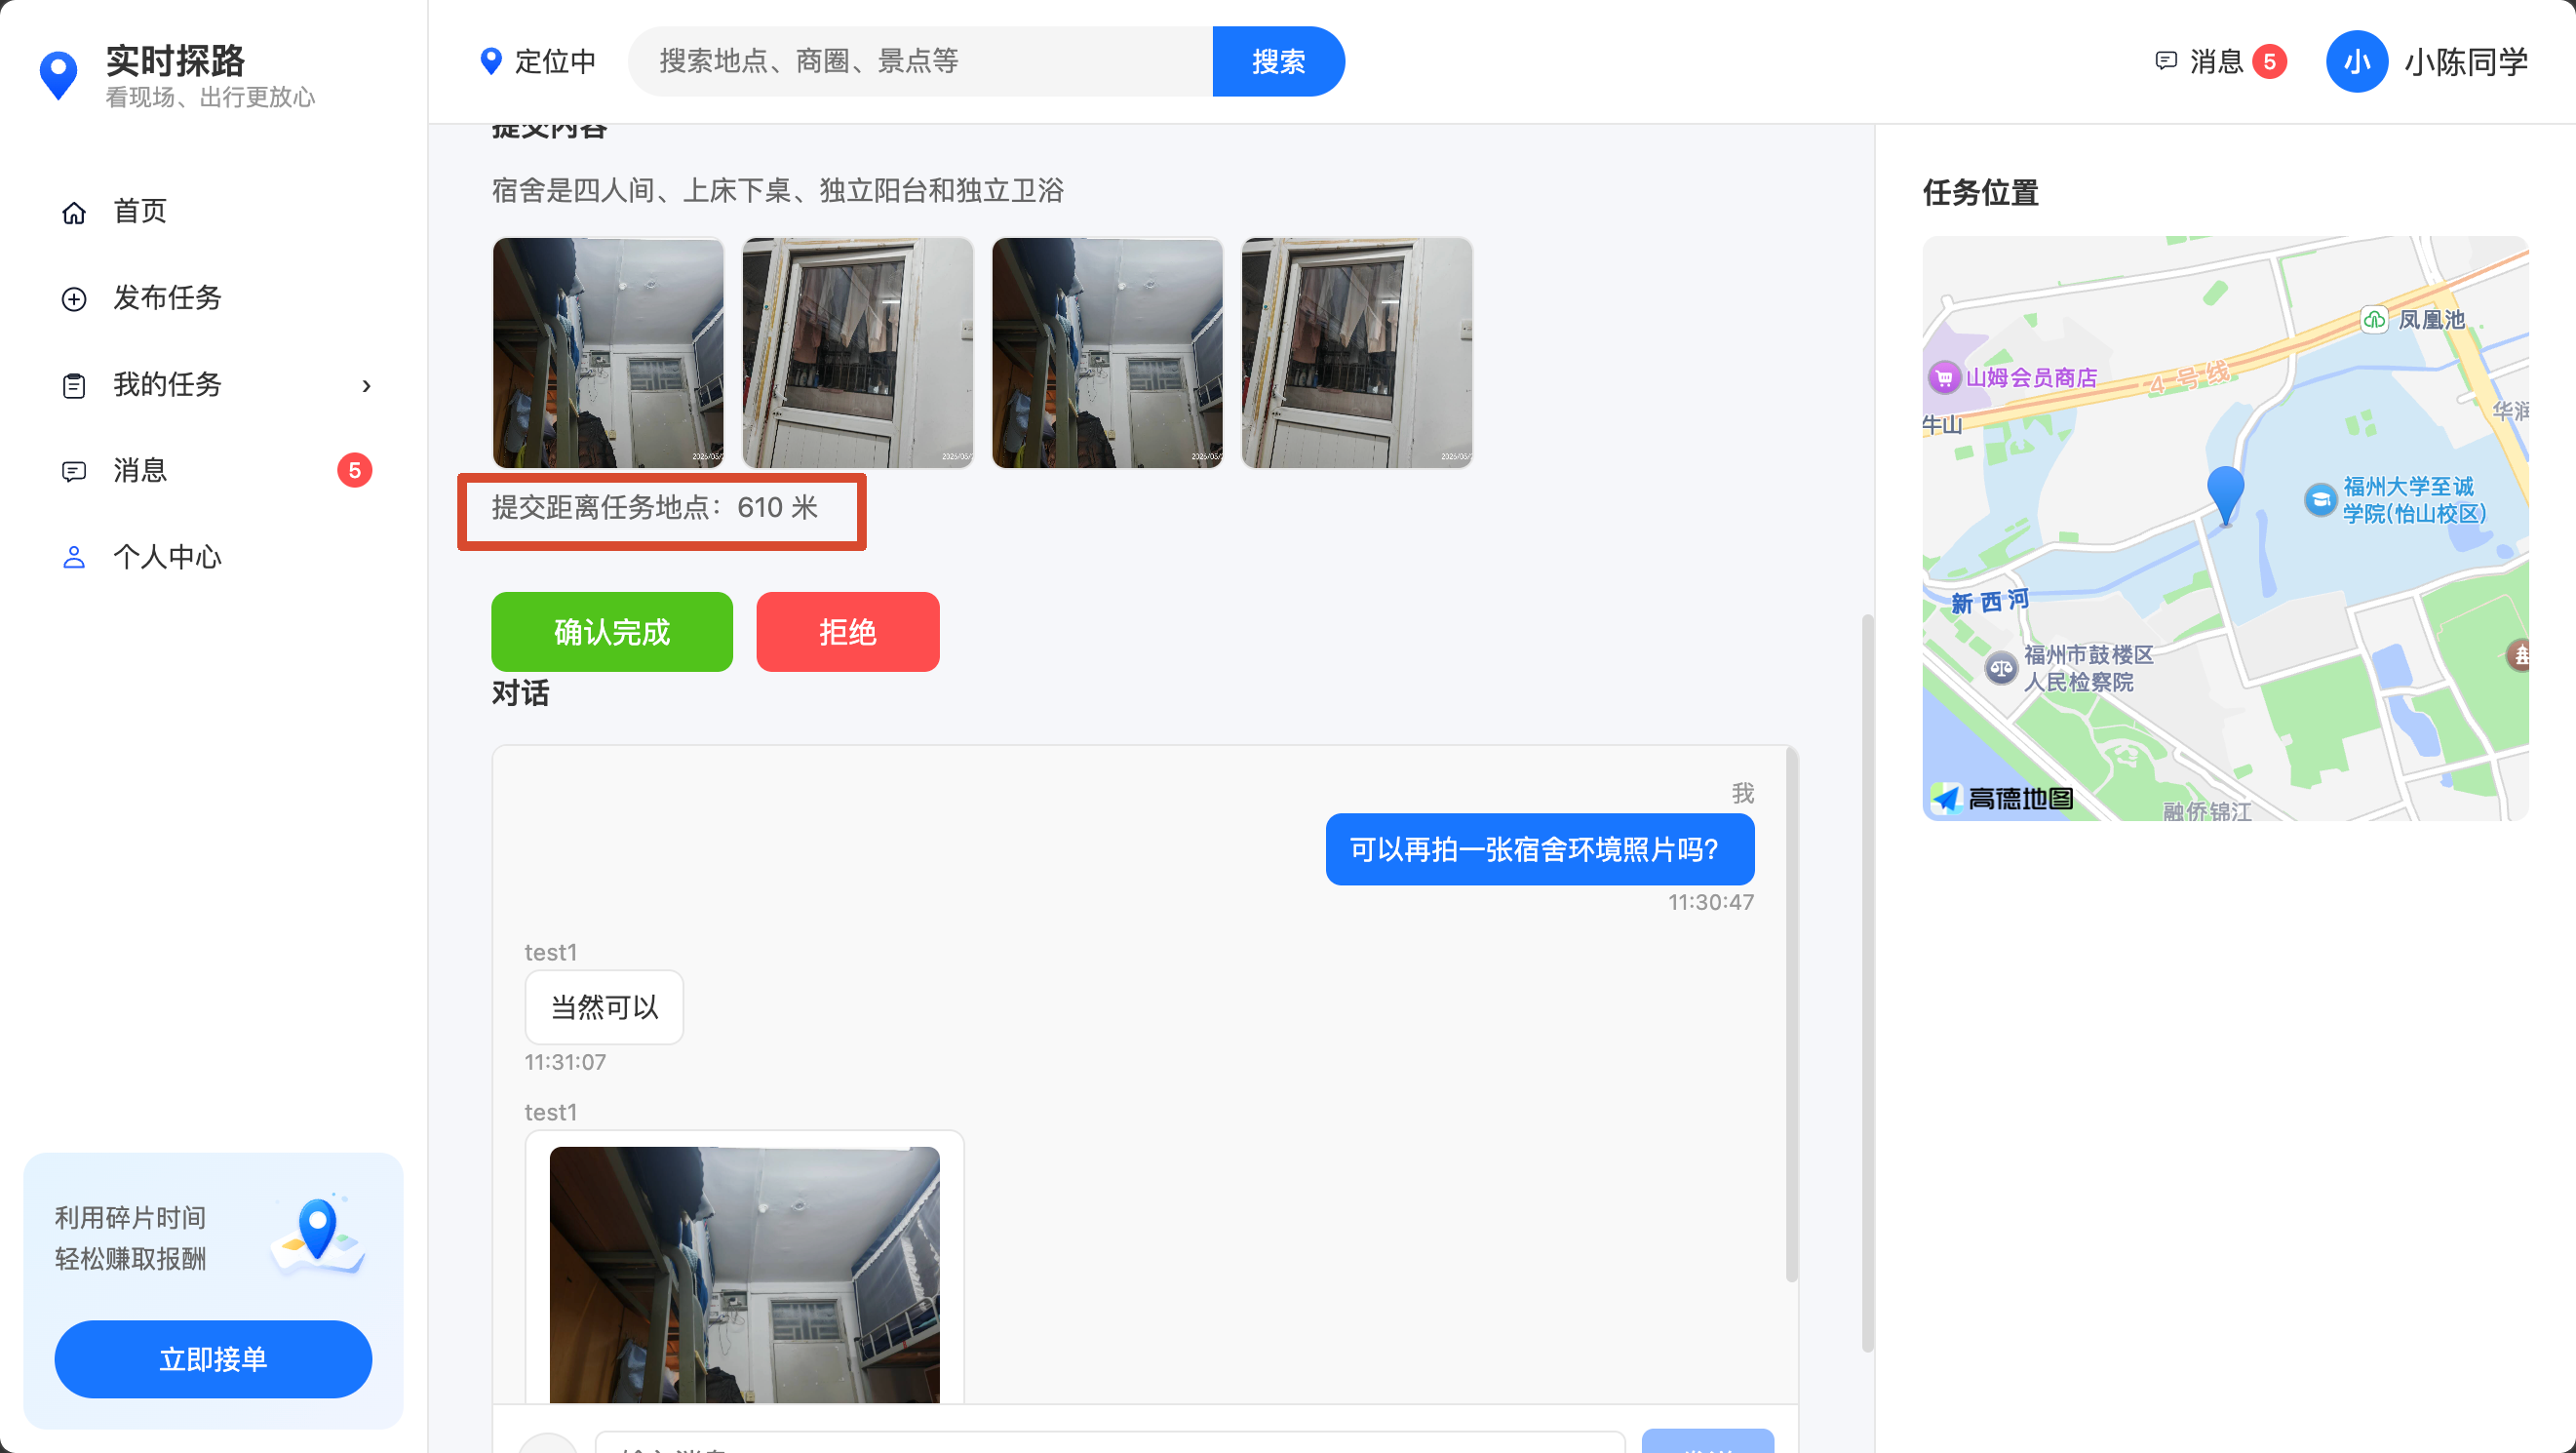
\includegraphics[width=\textwidth]{接单者需在任务点1公里范围内，用户可以通过聊天追加问题.png}
        \caption*{\small 实时聊天：追问细节，1公里范围校验}
    \end{subfigure}
    \hfill
    \begin{subfigure}[b]{0.4\textwidth}
        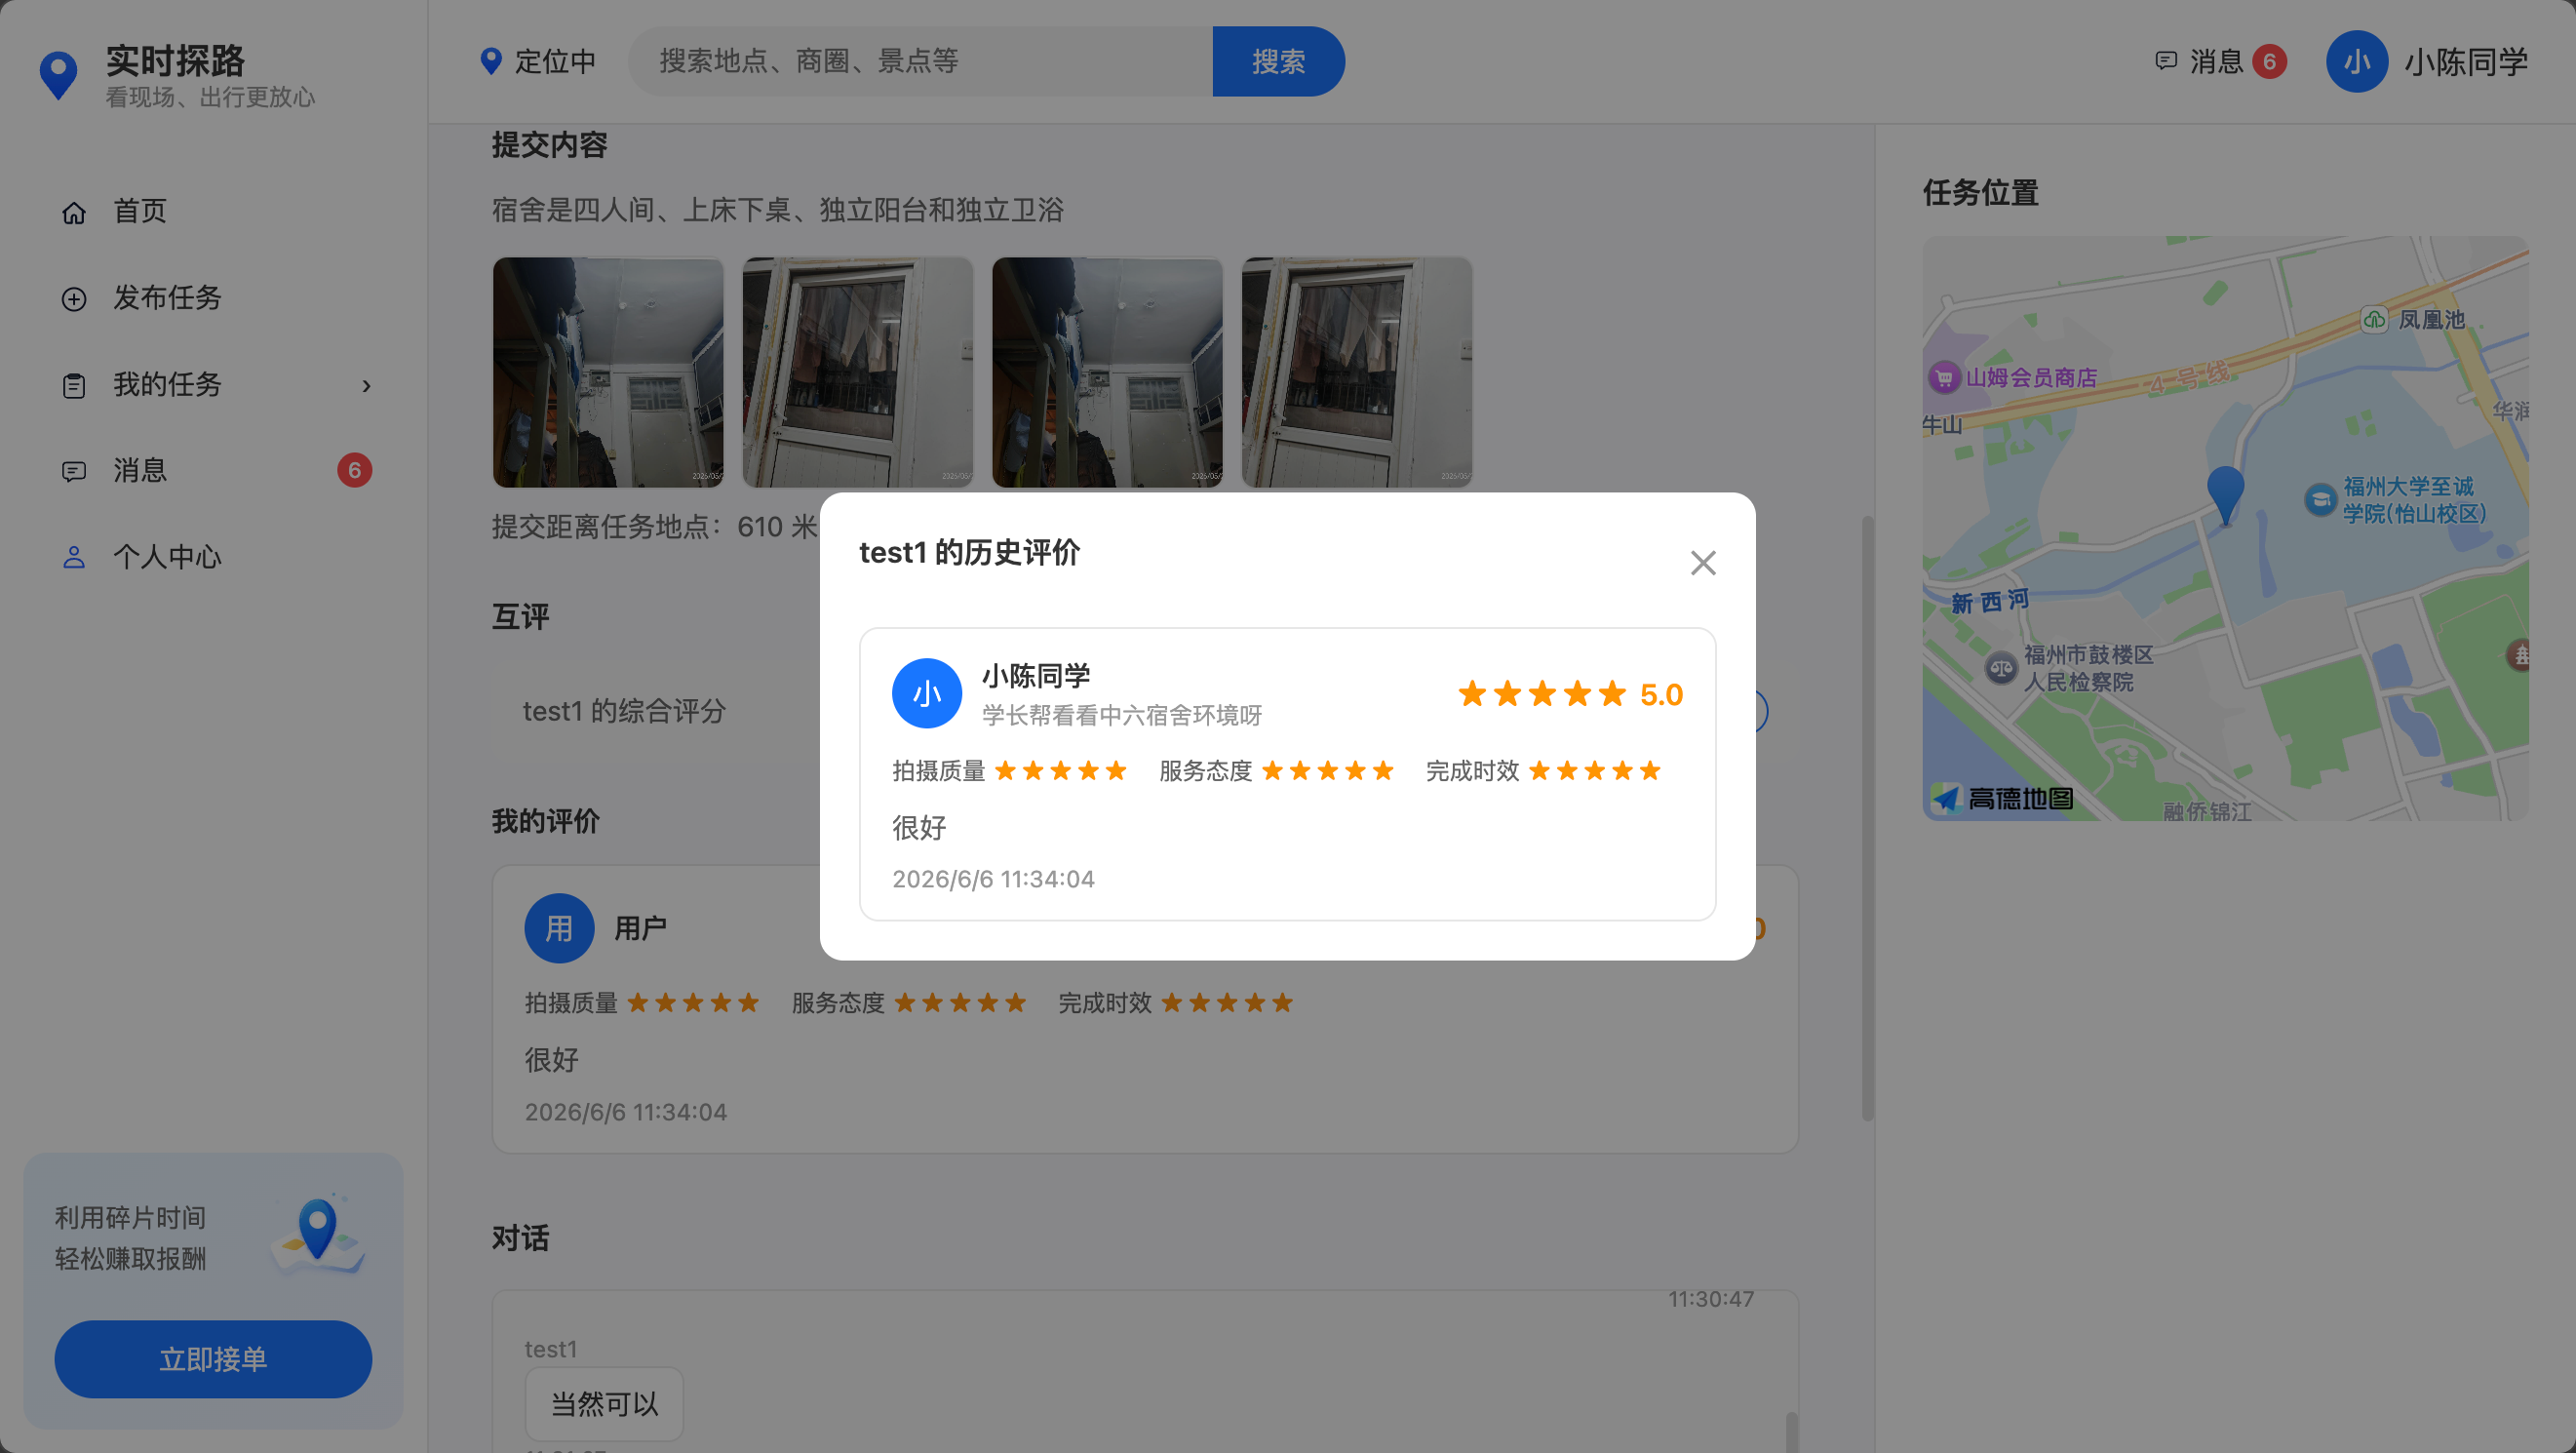
\includegraphics[width=\textwidth]{点击收货后可以给对方评价.png}
        \caption*{\small 确认收货后双向评价}
    \end{subfigure}
\end{figure}

\newpage

% ============================================================
%   第七章：运作流程
% ============================================================
\section{它是怎么运作的？}

\subsection{核心流程}

\begin{mdframed}[style=flowstyle]
\begin{center}
\renewcommand{\arraystretch}{1.8}
\begin{tabular}{ccc}
\textbf{① 发布任务} & \textbf{② 附近推送} & \textbf{③ 接单前往} \\
{\small 选地点+设赏金} & {\small 1km内用户可见} & {\small GPS校验位置} \\[8pt]
\textbf{④ 拍照提交} & \textbf{⑤ 确认收货} & \textbf{⑥ 赏金到账} \\
{\small 照片+文字描述} & {\small 满意确认/可追问} & {\small 实时结算到钱包} \\
\end{tabular}
\end{center}
\end{mdframed}

\subsection{资金安全}

\begin{mdframed}[style=flowstyle]
\begin{center}
发布任务时赏金\textbf{预冻结} $\longrightarrow$ 确认后\textbf{转给接单者} $\longrightarrow$ 过期/取消\textbf{自动退回}
\end{center}
\vspace{4pt}
{\small 发布者的钱不会凭空消失，接单者的劳动一定能得到回报。}
\end{mdframed}

\subsection{安全保障机制}

\begin{table}[H]
\centering
\renewcommand{\arraystretch}{1.4}
\begin{tabularx}{\textwidth}{>{\bfseries}l X}
\toprule
机制 & 说明 \\
\midrule
GPS定位校验 & 接单和提交时，设备定位需在任务地点\textbf{1000米}范围内 \\
资金托管 & 发布任务时悬赏金预冻结，确认后才发放给接单者 \\
时效保护 & 任务过期自动关闭并退款，不浪费发布者的钱 \\
自动确认 & 提交后24小时未操作自动确认支付，保护接单者权益 \\
隐私保护 & 禁止拍摄涉及他人隐私的内容，违规封号 \\
可拒绝/可放弃 & 发布者可拒绝不合格提交；接单者可放弃不想做的任务 \\
\bottomrule
\end{tabularx}
\end{table}

\newpage

% ============================================================
%   第八章：为什么需要实时探路
% ============================================================
\section{为什么需要「实时探路」？}

\subsection{现有方案的局限}

\begin{table}[H]
\centering
\renewcommand{\arraystretch}{1.4}
\begin{tabularx}{\textwidth}{>{\bfseries}l X X}
\toprule
现有方案 & 局限性 & 实时探路的优势 \\
\midrule
平台评论 & 好评可能是刷的，差评被淹没 & GPS定位验证，\textbf{确保真实} \\
小红书 & 广告软文太多，难辨真假 & 没有广告，\textbf{按需定制} \\
问朋友 & 朋友不一定在那个地方 & 总有人\textbf{正在那里} \\
看直播/短视频 & 博主选择性展示，不针对你的需求 & \textbf{按你的问题}回答 \\
自己跑一趟 & 时间成本、交通成本 & \textbf{几块钱}搞定 \\
看宣传图 & 精心修图，与实际不符 & \textbf{真实无滤镜}的现场 \\
\bottomrule
\end{tabularx}
\end{table}

\subsection{核心差异：GPS保证真实性}

\begin{mdframed}[style=infostyle]
实时探路和其他信息渠道最大的不同在于：

\vspace{6pt}
\textbf{每一条回答都经过定位验证}——接单者必须在任务地点1000米范围内才能接单和提交。

\vspace{6pt}
这意味着：
\begin{itemize}[leftmargin=1.5em, itemsep=2pt]
    \item 不可能远程编造虚假信息
    \item 不可能用旧照片冒充实时状况
    \item 你看到的，就是对方\textbf{此时此刻站在那里}拍给你的
\end{itemize}

\vspace{6pt}
一个很简单的诉求——"我只是想要一个真实的评价"——在信息过载的时代，反而变得很难。实时探路就是来解决这个问题的。
\end{mdframed}

\subsection{双赢模式}

\begin{mdframed}[style=hopestyle]
\textbf{对发布者：}
\begin{itemize}[leftmargin=1.5em, itemsep=2pt]
    \item 花几块钱，省下几小时和几十块油钱/路费
    \item 做出更好的出行决策，不再「赌运气」
    \item 保护家人的好心情——尤其是孩子的期待
\end{itemize}

\vspace{6pt}
\textbf{对接单者：}
\begin{itemize}[leftmargin=1.5em, itemsep=2pt]
    \item 碎片时间变现：逛街、等人、住酒店时顺手拍几张就能赚钱
    \item 零门槛：只要你在那个地方，拍张照就行
    \item 积累信用：好评率高的用户会被优先推荐高赏金任务
\end{itemize}
\end{mdframed}

\newpage

% ============================================================
%   第九章：结尾
% ============================================================
\section{让每一次出发都值得期待}

\begin{center}
\begin{mdframed}[style=endstyle]
\centering
\large

生活中太多「到了才知道」的遗憾：

\vspace{8pt}

排了一小时队才发现不值得；\\
开了半小时车才发现人太多；\\
定了酒店才发现和照片不一样；\\
带着满心期待出门，带着满心失望回家。

\vspace{12pt}

\textbf{实时探路}想做的很简单：

\vspace{8pt}

{\LARGE\bfseries 出发之前，先帮你看一眼。}

\vspace{12pt}

\normalsize
一笔小小的悬赏，\\
却能换回一整天的好心情。

\end{mdframed}
\end{center}

\vspace{1cm}

\begin{figure}[H]
    \centering
    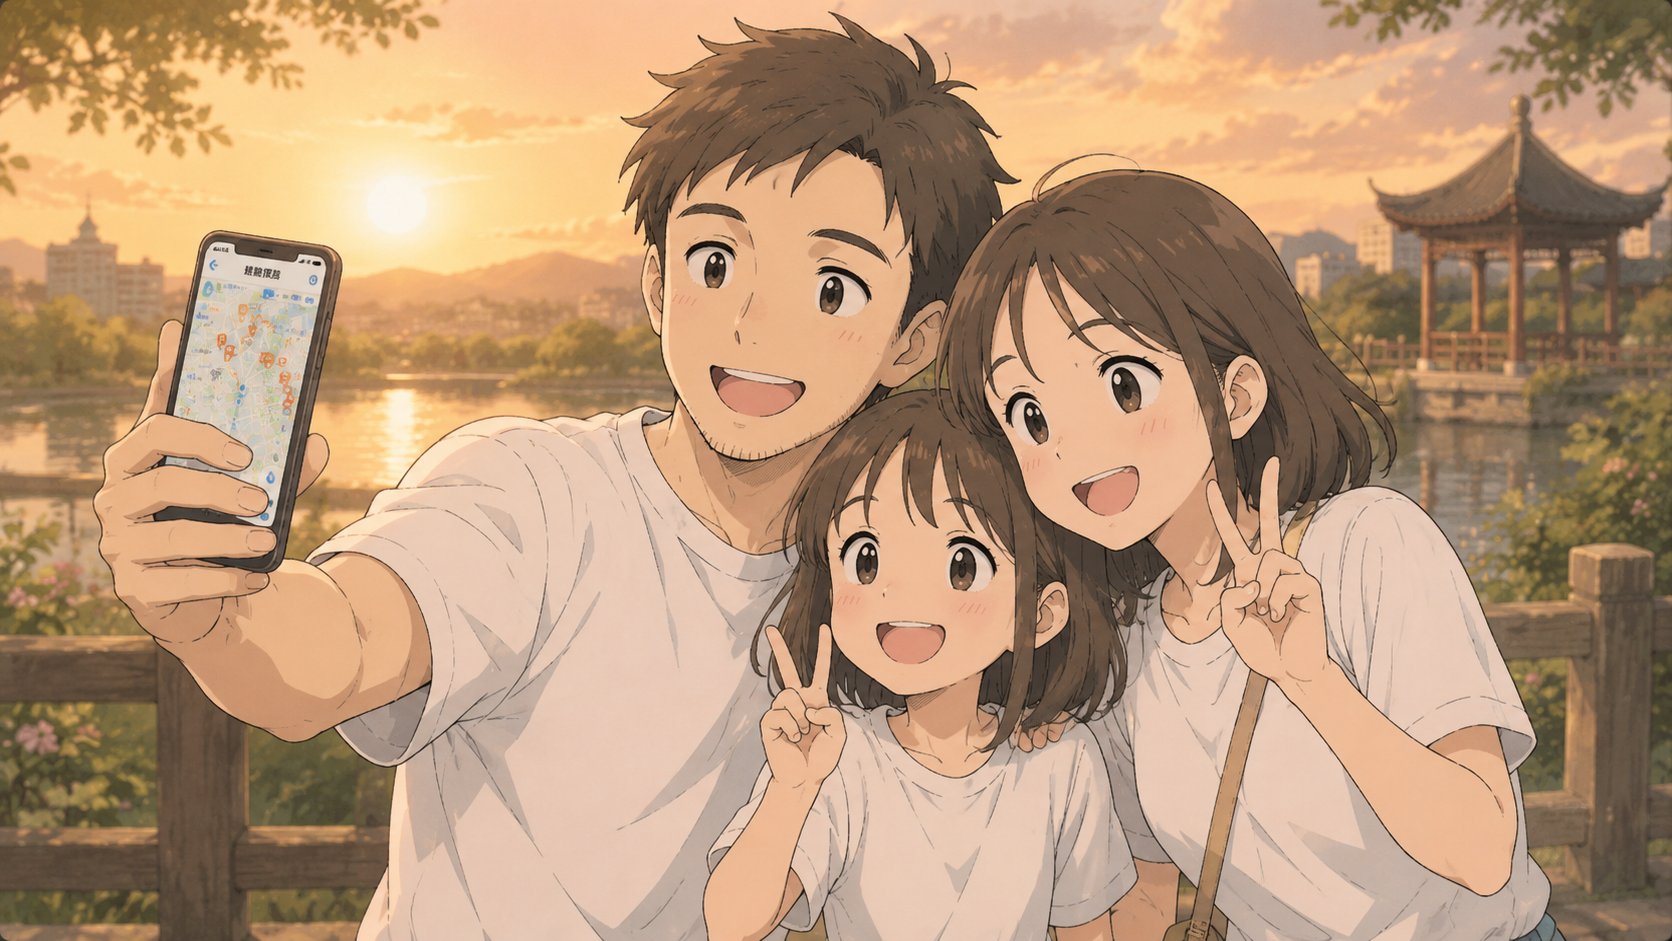
\includegraphics[width=0.5\textwidth]{20你们玩得很快乐.png}
    \caption*{\small 每一次出行，都应该是快乐的。}
\end{figure}

\end{document}
